%***********************************************************************
%* File            :    MAIN.tex
%*
%* HAUPTDOKUMENT
%*
%* Dieses Dokument bindet alle untergeordneten Dokumente
%* ein. Es wird beim Aufruf von pdflatex als Quelle angegeben.
%*
%* Autoren         :    Daniel Hering, Tobias Wartzek 
%*                      
%* Datum           :    05.12.2009
%***********************************************************************



\documentclass[12pt,a4paper,twoside,openright,index=totoc,listof=totoc,DIV15,BCOR=8.25mm,headinclude,footinclude=false,headsepline,notitlepage,numbers=noenddot,bibliography=totoc,headings=normal,parskip=full]{scrbook}

%************************************************************************
% Das Package muss leider hier eingebunden werden da sonst in den 
% Befehlen f�r hypersetup keinerlei Umlaute zur Verf�gung stehen
%************************************************************************

\usepackage[latin1]{inputenc}            % erlaubt direkte Eingabe Deutscher
                                         % Sonderzeichen in .tex Dateien
                                         %(latin1=iso8859-1 fuer Unix Editoren 
                                         % oder Windows Editoren die auch latin1
                                         % beherrschen)
                                         
%************************************************************************
% Dateiinfos eintragen (u.a. von hypersetup und f�r die Titelseite verwendet)
%************************************************************************
\usepackage{pdfpages}
% Titel der Arbeit 
\newcommand*{\doclongtitle}{Richtlinien f�r Abschlussarbeiten}

% Art der Arbeit (Diplomarbeit, Studienarbeit, Bachelorarbeit, etc.)
\newcommand*{\docsubject}{Masterarbeit}

% Name des Autors
\newcommand*{\docauthor}{Marian Walter}

% E-Mail Adresse des Autors
\newcommand*{\docauthoremail}{walter@hia.rwth-aachen.de}

% Schl�sselworte der Arbeit 
\newcommand*{\dockeywords}{MedIT Latex Studienarbeit Diplomarbeit Vorlage}

% Name des Betreuers
\newcommand*{\docsupervisor}{Dipl.-Ing. Mustermann}

\newcommand*{\docauthorfax}{+49 241 80-6-23211}
\newcommand*{\docauthorphone}{+49 241 80-23211}

% Bild auf der Titelseite
\newcommand*{\doctitlepic}{images/beispiel1}

% folgende Befehle nicht �ndern!!
\newcommand*{\dochomepage}{www.medit.hia.rwth-aachen.de}
\newcommand*{\docshorttitle}{\doclongtitle}

%**********************************************
%* Pakete (HEADER)                           *
%**********************************************

%************************************************************************
%* File            :    HEADER.tex
%*
%* Einbinden der erforderlichen Package-Dateien.
%* Definition des PDF-Infoblocks (im Acrobat Reader unter
%* Datei/Dokumenteigenschaften/Uebersicht)
%*
%* Autor  	       :    Daniel Hering, Tobias Wartzek
%* Datum           :    07.12.2009
%************************************************************************

\usepackage[T1]{fontenc}
\usepackage{lmodern}
\usepackage{helvet}
%\usepackage{palatino}
%\usepackage{times}


\usepackage[ngerman]{babel}              % Deutsche Silbentrennung ...
                                         % Sollte direkt nach documentclass 
                                         % geladen werden.
\usepackage{scrpage2}                    % Kopf- und Fusszeilen
\usepackage{ifpdf}                       % PDF Ausgabe oder nicht ?
                                         % Dieses Paket muss ueber dem graphicx
                                         % Paket stehen.

\usepackage{color}                       % farbig drucken                      
\usepackage{graphicx}                    % alle mgl. Arten von Bildern einbinden
\usepackage{subfigure}
\usepackage{eso-pic}										 % mehrschichtige Seitenlayouts
\usepackage{tikz}												 % Zeichenpaket und Optionen f�r Bilder.

%******************************************************************************************
% Wenn Matlab Plots erstellt werden sollen, muss das folgende package eingebunden werden. *
% Allerdings kann es vorkommen, dass das package noch nicht installiert ist, so dass *
% dies nachinstalliert werden m�sste.

%\usepackage{pgfplots}							 % Einbinden von Matlab-Plots      		*
%\pgfplotsset{compat=newest}
%\usetikzlibrary{plotmarks}
%******************************************************************************************

% Pakete f�r Tabellen
\usepackage{tabularx}                    % Breite Tabellen (seitenbreite)
\usepackage{multicol}                    % \multicols: Mehrspaltig auf einer Seite
\usepackage{hhline}                      % schoenere Doppellinien fuer Tabellen
\usepackage{longtable}                   % Lange Tabellen
\usepackage{multirow}                    % Mehrzeilige Tabellenzellen
\usepackage{colortbl}										 % Farbige Tabellenzeilen

\usepackage[gennarrow]{eurosym}          % Das Eurosymbol - benutzen mit \EUR{1,00} oder \euro{}
\usepackage{amsmath}                     % mathematische Sonderzeichen
\usepackage{amsxtra}
\usepackage{amssymb}                   	 % Zusaetzliche mathematische Symbole
\usepackage{units}											 % Verwendung: 
\usepackage{acronym}										 
\usepackage{scrhack}										 % Beseitigt Inkompatibilit�ten zwischen Komascript und Listings-Paket
\usepackage{listings}										 % Darstellung von Programmcode als Listing
\usepackage{url} 
\usepackage[pdfpagelabels]{hyperref}     % Konfiguration ueber hypersetup
                                         % hyperref sollte als eines der
                                         % letzten Pakete eingebunden werden

\usepackage{ragged2e}										 % Links-/rechtsb�ndig und trotzdem passende Zeilenumbr�che





\newcommand{\changefont}[3]{
	\fontfamily{#1} \fontseries{#2} \fontshape{#3} \selectfont}
\changefont{ptm}{m}{n}

%%%%%%%%%%%%%%%%%%%%%%%%%%%%%%%%%%%%%%%%%%%%%%%%%%%%%%%%%%%%%%%%%%%%%%%%%%%%%%%%%%%%%%%
%%%%%%%%%%%%%%%%%%%%%%%%%%%%%%%%%%%%%%%%%%%%%%%%%%%%%%%%%%%%%%%%%%%%%%%%%%%%%%%%%%%%%%%
%**************************************************************************************
%*     																																								*
%* Ab hier folgen Definitionen einiger Einstellungen die nicht 								  			*
%* vom Benutzer ge�ndert werden m�ssen. 																		  				*
%* 																																						  			*
%**************************************************************************************

\definecolor{rwthblue}{rgb}{0,0.4,0.8}    % Das RWTH-Blau
\definecolor{hellgrau}{rgb}{0.9,0.9,0.9} 	% hellgrau

%************************************************************************
%*																																			*
%* F�r die Ausgabe mit pdflatex n�tige Befehle zur sinnvollen Benutzung	*
%* des Hyperref-Pakets. Auch hier sind normal keine Anpassungen durch 	*
%* den Benutzer n�tig 																									*
%*																																			*
%************************************************************************


\ifpdf
  % \Htmlfalse
  \pdfoutput=1

  \hypersetup{
                pdftitle={\docshorttitle, RWTH Aachen},
                pdfauthor={\docauthor},
                pdfsubject={\docsubject},
                pdfkeywords={\dockeywords},
                pdfpagemode={UseNone},
                plainpages={false},
                colorlinks=true,  % die Option colorlinks schaltet um zwischen "Rahmen
                linkcolor=black,	% um link" -> false und "Text farbig" -> true 
				        citecolor=black,  % daher sind die Farbdefinitionen n�tig um Links nicht
				        filecolor=black,	% im Text hervorzuheben. (entw. weisse Rahmen oder
        				urlcolor=black		% eben schwarzer Text)
   }      
\fi


%*************************************************************
% Die folgenden zwei Zeilen werden ben�tigt sofern Matlab-	 *
% Plots eingebunden werden sollen														 *
%*************************************************************

\newlength\fheight											% ben�tigt zur Einbindung von Matlab-Plots 
\newlength\fwidth												% auskommentieren bei nichtbenutzen


%****************************************************************
% Die folgenden zwei Zeilen �ndern die Gr��e der 	        	    *
% Unterschriften um eine klare Abgrenzung zum Text zu erreichen *
%****************************************************************

\setkomafont{caption}{\small}									% Bild-/Tabellenunterschrift �ndern
\setkomafont{captionlabel}{\small\bfseries}


%*******************************************************************
%* Abb. statt Abbildung	/ Tab. statt Tabelle											 *
%*******************************************************************
\addto\captionsngerman{
\renewcommand{\figurename}{Abb.}
\renewcommand{\tablename}{Tab.}
} 


%*******************************************************************
%* Vertikaler Abstand vor Chapter �berschrift �ndern  						 *
%*******************************************************************
\renewcommand {\chapterheadstartvskip}{\vspace*{-\topskip}} 




%*************************************************************
%*************************************************************
%*																													**
%* 					Beginn des Dokuments 						  							**
%*																													**
%*************************************************************
%*************************************************************

\begin{document}
\begin{sloppypar}                       % sch�ner Blocksatz trotz langer Worte



%*************************************************************
%																														 *
%										 ENDE ALLER DEFINITIONEN 								 *
%																														 *
%*************************************************************


\frontmatter    												%r�mische Nummerierung aktivieren
%***********************************************************************
%* File            :    titel2.tex
%*
%* Titelseite 		 
%*
%* Autor           :    Daniel Hering
%***********************************************************************

\newcommand{\defaultarraystretch}{\arraystretch}

\begin{titlepage}
\enlargethispage{31mm}
%***********************************************************************
%* Definition der Kopfzeile																						 *
%***********************************************************************
\vspace*{-3cm}
\hspace*{-1.8em}
\begin{tabularx}{19cm}{Xl@{}}
\textsf{\textbf{\LARGE{\docsubject}}} & %
\includegraphics[height=45pt]{images/RWTH_Aachen_University}
\\
\mbox{\vspace{-10mm}\colorbox{rwthblue}{\hspace{18.4cm}}
\rule{0pt}{10pt}}
%\vspace{-10mm}\colorbox{rwthblue}{\hspace{12.7cm}}  {
\includegraphics[height=30pt]{images/medit_l_m_blau_meditheadfoot}}
\end{tabularx}

%***********************************************************************
%* Ende der Definition der Kopfzeile																	 *
%***********************************************************************
\vspace*{15mm}
\par
\begingroup
\huge
\leftskip20pt
\noindent \textsf{\LARGE\docauthor\\ 
\textbf{\huge \docshorttitle}}
\par
\endgroup
\vfill % F�llt die Seite vertikal auf 

%***********************************************************************
%* Hier eine zur Diplomarbeit geh�rende Grafik einbinden 							 *	
%***********************************************************************
% 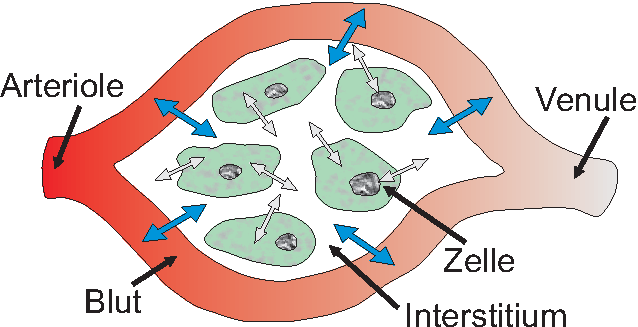
\includegraphics[width=190mm]{images/beispiel1}\vspace{10pt}

\AddToShipoutPicture*{
     \parbox[b][\paperheight]{\paperwidth}{%       
       \vfill
        \centering
        \begin{tikzpicture}[overlay]%
       		  %\draw[help lines] (0,0) grid (10,20);
            \node (0,0) [opacity=0.4]{%
             \hspace{-8,25mm}\includegraphics[width=10cm, height=10cm,keepaspectratio]{\doctitlepic}};%
         \end{tikzpicture}
       \vspace{32.35em}
     }}







\renewcommand{\arraystretch}{1.3}
\hspace*{-1.8em}
\begin{tabularx}{19cm}{Xl}
\multicolumn{2}{l}{\colorbox{rwthblue}{\hspace{18.4cm}}}\\
\multicolumn{2}{l}{\textsf{\textbf{LEHRSTUHL F�R MEDIZINISCHE INFORMATIONSTECHNIK}}}\\
\multicolumn{2}{l}{\textsf{{Fakult�t f�r Elektrotechnik und Informationstechnik, RWTH Aachen}}}\\
\multicolumn{2}{l}{\textsf{Univ.-Prof. Dr.-Ing. Dr. med. Steffen Leonhardt}}\\
\textsf{Betreuer-/in: \docsupervisor} & \\ 
\textsf{Datum: \today} & \multirow{-2}*~%{
\includegraphics[height=30pt]{images/medit_l_m_blau_meditheadfoot}} \\
\end{tabularx}%}
\renewcommand{\arraystretch}{\defaultarraystretch}

\thispagestyle{empty}
\cleardoublepage

\end{titlepage}

%%***********************************************************************
%* File            :    titel.tex
%*
%* Titelseite 		 
%*
%* Autor           :    Daniel Hering
%***********************************************************************



\let\savedbaselinestretch=\baselinestretch    % Probleme mit geandertem 
                                              % baselinestretch umgehen
\renewcommand{\baselinestretch}{1}%
\begin{titlepage}

%***********************************************************************
%* Definition der Kopfzeile																						 *
%***********************************************************************

\titlehead{\vspace*{-15mm}\underline{\parbox[b]{\textwidth}{
\includegraphics[height=24pt]{images/rwth_logo_blau_rechts}\parbox[b]{0.632\textwidth}{\raggedleft\textcolor{rwthblue}{\footnotesize{HELMHOLTZ-INSTITUT F�R BIOMEDIZINISCHE TECHNIK\\DER RWTH AACHEN}}}
\includegraphics[height=24pt]{images/hia_logo_blau}}}\\\underline{\parbox[b]{\textwidth}{LEHRSTUHL F�R MEDIZINISCHE INFORMATIONSTECHNIK\\Univ.-Prof. Dr.-Ing. Dr. med. Steffen Leonhardt}}}

%***********************************************************************
%* Ende der Definition der Kopfzeile																	 *
%***********************************************************************

\subject{\vspace*{2\baselineskip}}
\title{\docshorttitle}
\author{
  \parbox{.8\linewidth}{%
     \centering\docauthor\\%
\vspace{0.7em}
\large Betreuer/-in: \docsupervisor\\
 \date{\large \today}
}
}%

\publishers{\small\vspace*{\stretch{1000}}%
  \parbox{\linewidth}{%
  \vspace{10cm}
    Pauwelsstra�e 20\\%
    D-52074 Aachen\\%
    Telefon: +49 (0)241 80 -23211\\%
    Fax: +49 (0)241 80 -82442\\%
    E-Mail: medit@hia.rwth-aachen.de\\%
  }%
  \vspace*{-\stretch{1}}%
}
\maketitle
\thispagestyle{empty}
\cleardoublepage
\let\baselinestretch=\savedbaselinestretch%
\end{titlepage}



\cleardoubleemptypage


%**************
%* Danksagung *
%**************

\chapter{Danksagung}
\thispagestyle{empty}
<!-- start slipsum code -->
Your bones don't break, mine do. That's clear. Your cells react to bacteria and viruses differently than mine. You don't get sick, I do. That's also clear. But for some reason, you and I react the exact same way to water. We swallow it too fast, we choke. We get some in our lungs, we drown. However unreal it may seem, we are connected, you and I. We're on the same curve, just on opposite ends.

Do you see any Teletubbies in here? Do you see a slender plastic tag clipped to my shirt with my name printed on it? Do you see a little Asian child with a blank expression on his face sitting outside on a mechanical helicopter that shakes when you put quarters in it? No? Well, that's what you see at a toy store. And you must think you're in a toy store, because you're here shopping for an infant named Jeb.

You see? It's curious. Ted did figure it out - time travel. And when we get back, we gonna tell everyone. How it's possible, how it's done, what the dangers are. But then why fifty years in the future when the spacecraft encounters a black hole does the computer call it an 'unknown entry event'? Why don't they know? If they don't know, that means we never told anyone. And if we never told anyone it means we never made it back. Hence we die down here. Just as a matter of deductive logic.
<!-- end slipsum code -->
\cleardoubleemptypage

%************************************************
%* Erkl�rung (hier muss nichts ge�ndert werden) *
%************************************************

%\chapter*{Erkl�rung}
%\thispagestyle{empty}
%\hypertarget{hypsec:erklaerung_der_selbstst}{}%
%
%Ich versichere hiermit, dass ich die vorliegende Arbeit selbstst�ndig
%und ohne Benutzung anderer als der angegebenen Hilfsmittel angefertigt
%habe. Alle Stellen, die w�rtlich oder sinngem�� aus
%ver�ffentlichten und nicht ver�ffentlichten Schriften entnommen
%sind, wurden als solche kenntlich gemacht.\\[3cm]
%
%\begin{tabularx}{\textwidth}{lXl}
%  \rule{5cm}{0.4pt} & & \rule{5cm}{0.4pt}\\
%  Ort, Datum & & Unterschrift
%\end{tabularx}
%\includepdf[angle=90,landscape]{Testbild.png}
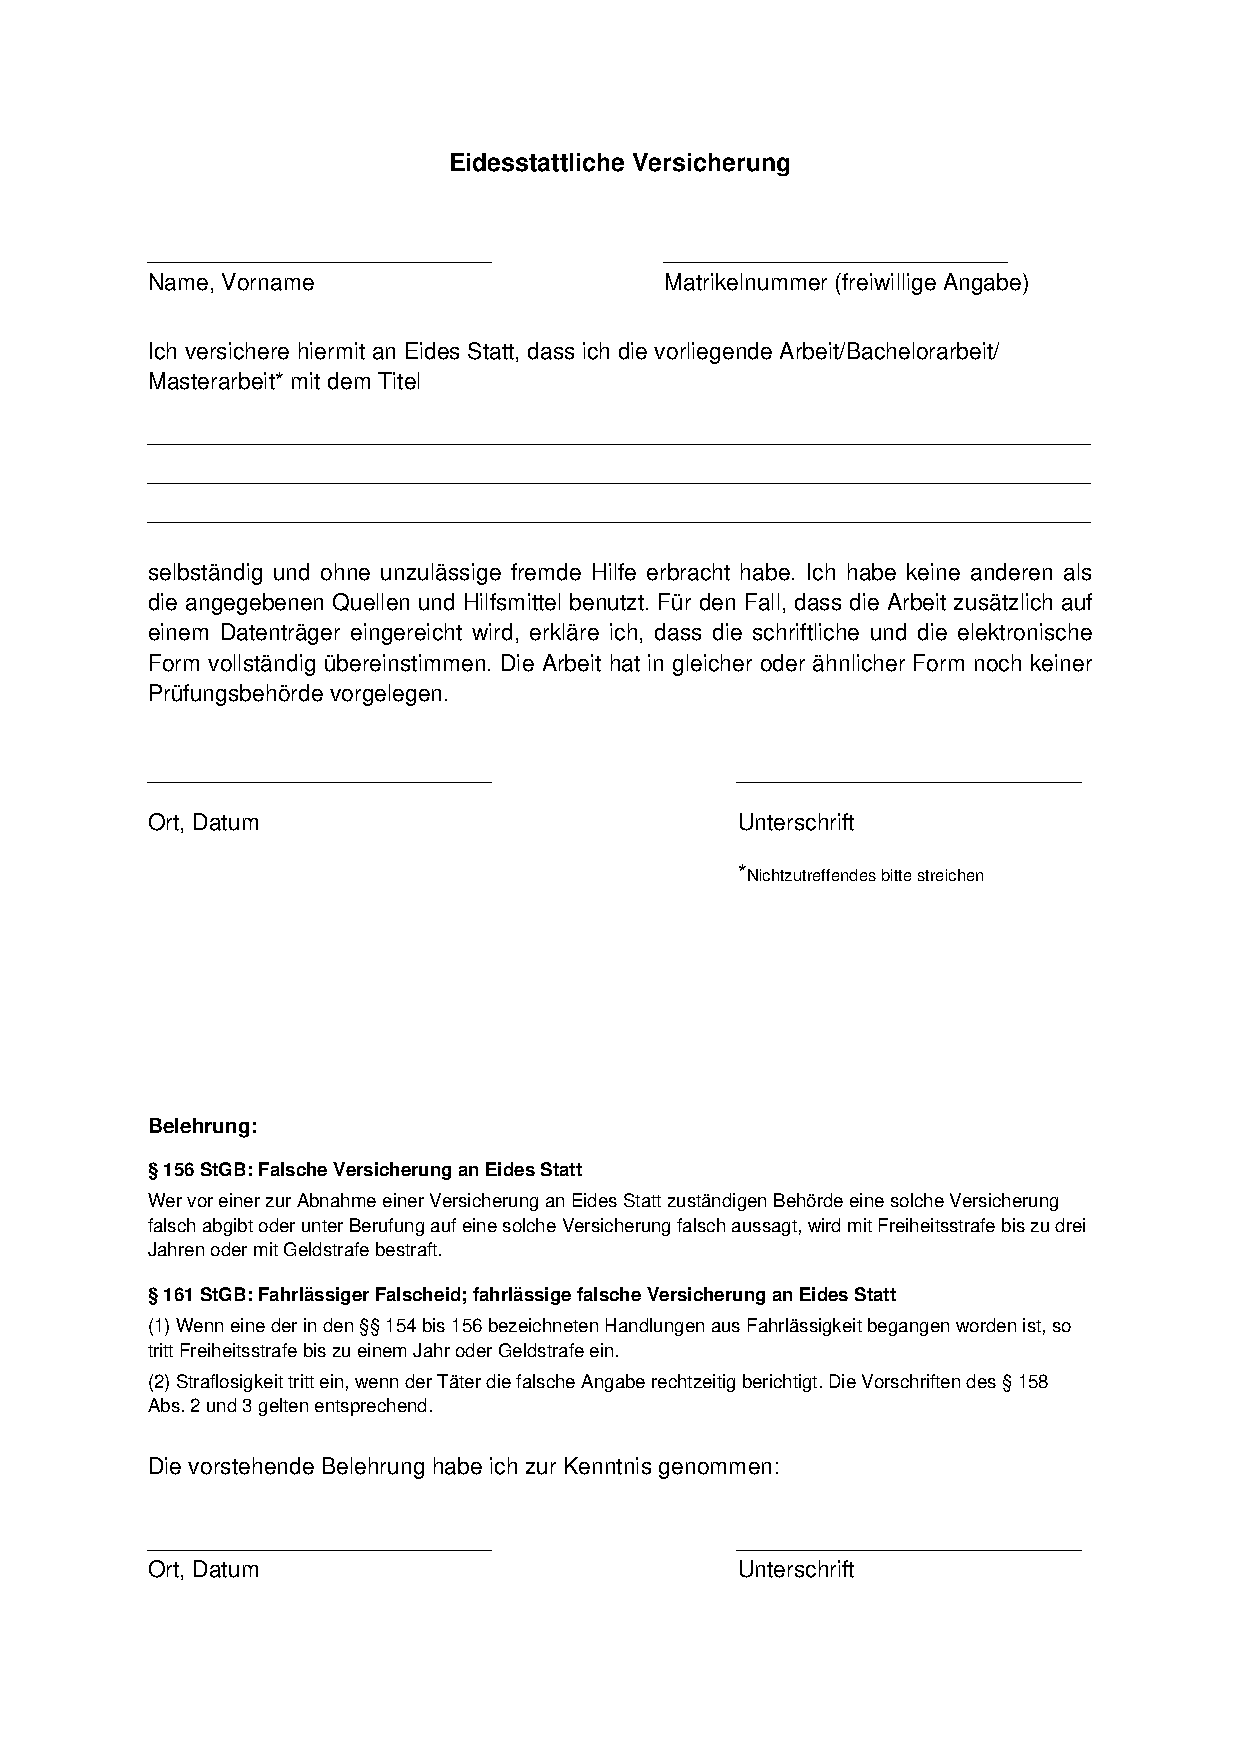
\includepdf{images/Formular_Eidesstattliche_Versicherung_neu}

%\begin{figure}[!ht]
%  \centering
%   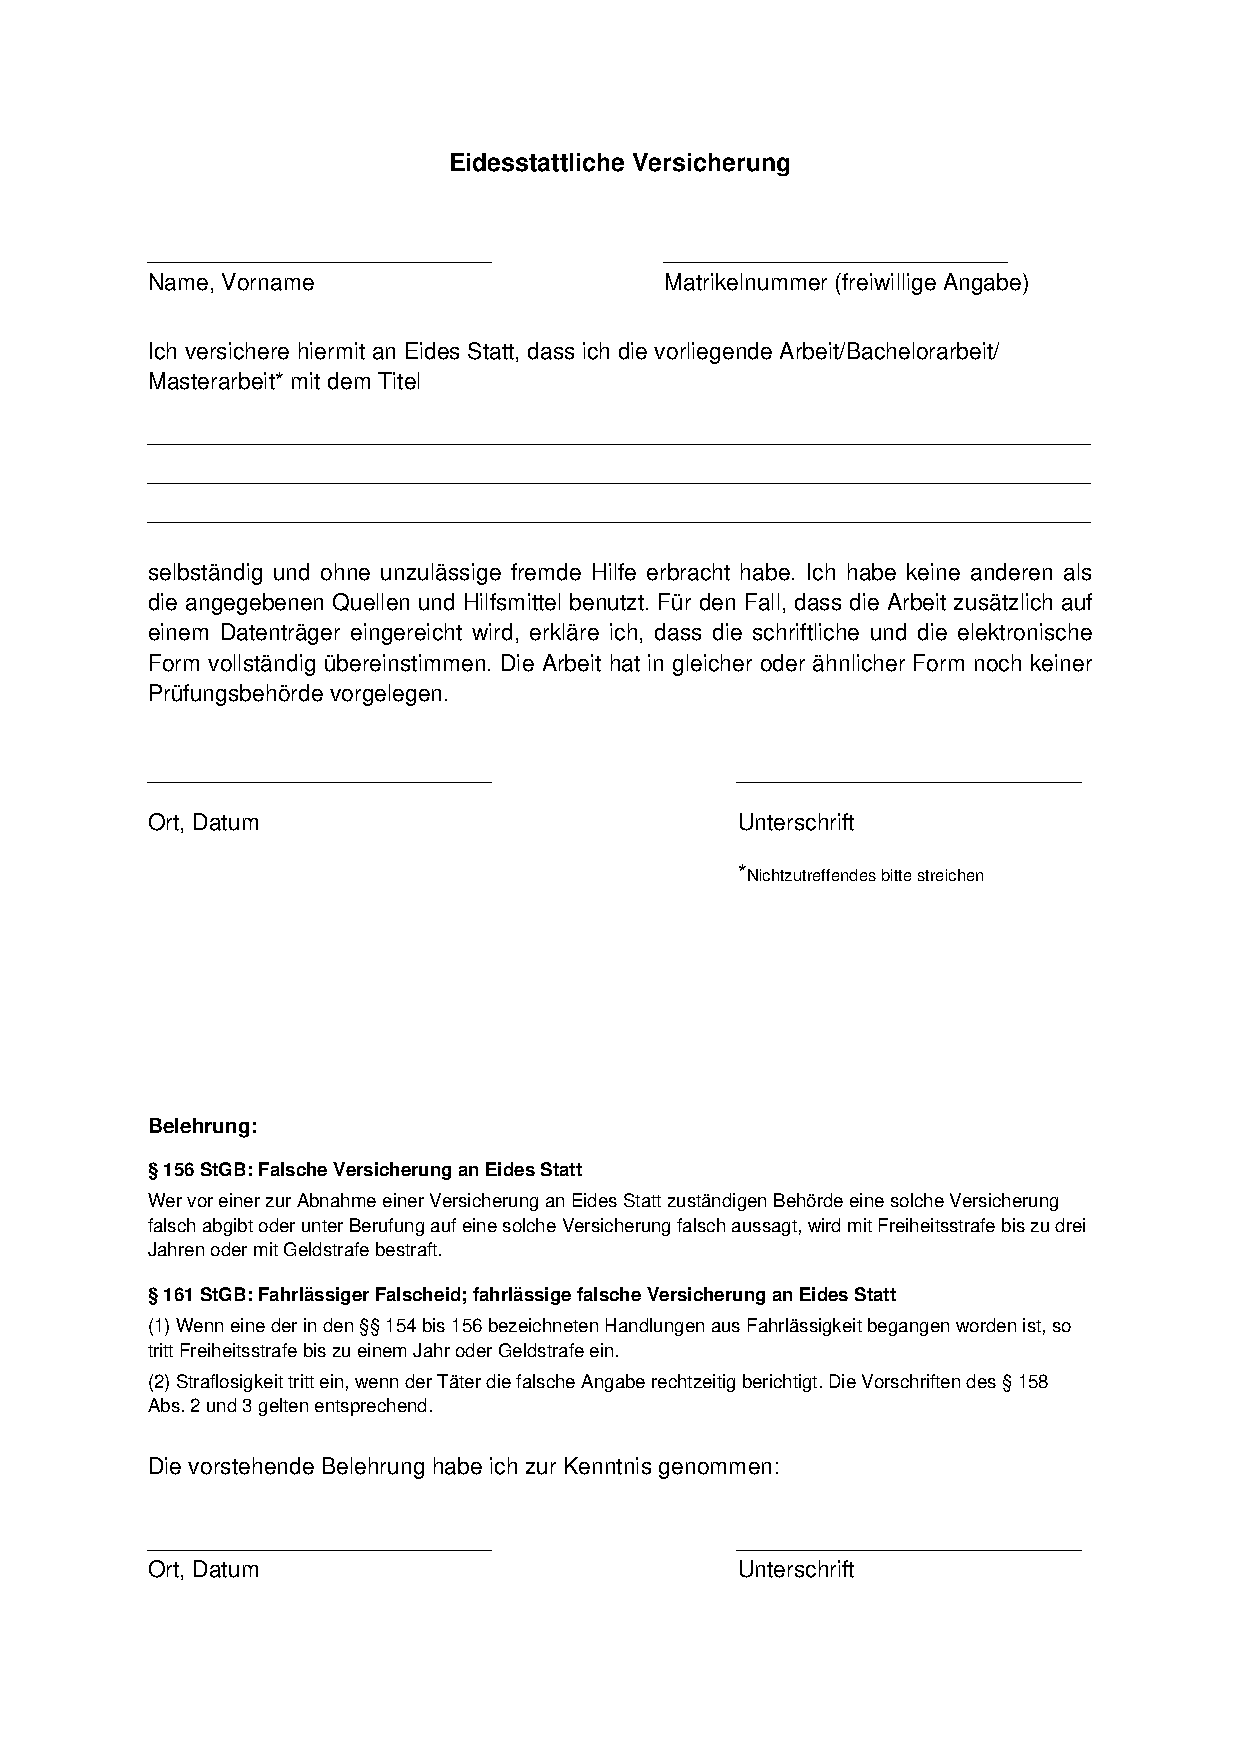
\includegraphics[scale=1]{images/Formular_Eidesstattliche_Versicherung_neu}
%   % Die folgende Anweisungen bindet die Grafik nocheinmal zus�tzlich
%   % als Dateianhang ein. Das hat den Vorteil, dass sie einfach aus dem pdf zur
%   % wieterverwendung extrahierbar ist und der Autor (author) mit angegeben
%   % werden kann. Leider ist die Grafik dadurch auch gleich zweimal im pdf
%   % enthalten und verbraucht dadurch doppelt Platz.
%   % \textattachfile[mimetype=application/pdf,print=false,author=\docauthor,description=\figurename~\ref{fig:beispiel1}]{beispiel1.pdf}{}
%  %% Reihenfolge der Befehle wichtig: zuerst die \caption, danach das \label
%  \label{fig:EidesstattlicheVersicherung}
%\end{figure}

\cleardoubleemptypage

%************
%* Abstract *
%************

\chapter{Zusammenfassung}

<!-- start slipsum code -->
Now that we know who you are, I know who I am. I'm not a mistake! It all makes sense! In a comic, you know how you can tell who the arch-villain's going to be? He's the exact opposite of the hero. And most times they're friends, like you and me! I should've known way back when... You know why, David? Because of the kids. They called me Mr Glass.

You see? It's curious. Ted did figure it out - time travel. And when we get back, we gonna tell everyone. How it's possible, how it's done, what the dangers are. But then why fifty years in the future when the spacecraft encounters a black hole does the computer call it an 'unknown entry event'? Why don't they know? If they don't know, that means we never told anyone. And if we never told anyone it means we never made it back. Hence we die down here. Just as a matter of deductive logic.

Now that we know who you are, I know who I am. I'm not a mistake! It all makes sense! In a comic, you know how you can tell who the arch-villain's going to be? He's the exact opposite of the hero. And most times they're friends, like you and me! I should've known way back when... You know why, David? Because of the kids. They called me Mr Glass.
<!-- end slipsum code --> 


\cleardoubleemptypage
\thispagestyle{empty}
\cleardoubleemptypage

%**********************
%* Inhaltsverzeichnis *
%**********************


\addcontentsline{toc}{chapter}{Inhaltsverzeichnis} % Eintrag im Inhaltsverzeichnis erstellen
\tableofcontents                        % Inhaltsverzeichnis anlegen
\cleardoubleemptypage



%*********************
%* Symbolverzeichnis *
%********************

\chapter*{Symbolverzeichnis}										% da *-Variante m�ssen Kopfzeilen und TOC-Eintrag von Hand generiert werden
\markboth{Symbolverzeichnis}{Symbolverzeichnis} 				% Kopfzeile manuell anpassen 
\addcontentsline{toc}{chapter}{Symbolverzeichnis}				% TOC-Eintrag



\section*{Abk�rzungen}

%* Benutzung der Acronym-Umgebung
%* \acrodef{Name zum aufrufen im Dokument}[gew�nschte Abk�rzung]{ausgeschriebener Begriff}
%* \ac{Name} zur Verwendung im Dokument - beim 1.maligen Verwenden wird der ausgeschriebene
%* Begriff mit der Abk�rzung dahinter in Klammern gesetzt, danach nur noch die Abk�rzung

\acrodef{H2O}[$\mathrm{H_2O}$]{Wasser}
\acrodef{RWTH}[RWTH Aachen]{Rheinisch-Westf�lische Technische Hochschule Aachen}
\acrodef{DPO}[DPO]{Diplompr�fungsordnung}

%* \acs{Name} ruft explizit die Abk�rzung auf.
%* \acl{Name} ruft explizit den ausgeschriebenen Begriff auf.

\begin{tabularx}{\textwidth}{p{.18\textwidth}X}
\acs{H2O} & \acl{H2O} \\
\acs{RWTH} & \acl{RWTH}\\
\acs{DPO} & \acl{DPO}\\
\end{tabularx}

\section*{Physikalische Gr��en}

\begin{tabularx}{\textwidth}{p{.18\textwidth}Xp{.1\textwidth}}
$\mathrm{v}$ & Geschwindigkeit & $\frac{km}{h}$ \\
$\mathrm{t}$ & Zeit & $h$\\
\end{tabularx}

\section*{Mathematische Gr��en}

\begin{tabularx}{\textwidth}{p{.18\textwidth}X}
$\mathrm{M}$ & mathematische Beispielgr��e \\
\end{tabularx}

\section*{Indizes}

\begin{tabularx}{\textwidth}{p{.18\textwidth}X}
$k$ & Anzahl der Proze�schritte \\
$P_{1}...P_{n}$ & Proze�schritt $P_{1}$ bis $P_{n}$\\
$V_{Ziel}$ &  Zielvektor\\
\end{tabularx}

\section*{Konstanten}

\begin{tabularx}{\textwidth}{p{.18\textwidth}X}
$\pi$ & 3.141592653589 \\
\end{tabularx}
\cleardoubleemptypage

\mainmatter							% Arabische Nummerierung, Beginn des Hauptteils

%**************
%* Einleitung *
%**************

\chapter{Einleitung}

<!-- start slipsum code -->
Now that we know who you are, I know who I am. I'm not a mistake! It all makes sense! In a comic, you know how you can tell who the arch-villain's going to be? He's the exact opposite of the hero. And most times they're friends, like you and me! I should've known way back when... You know why, David? Because of the kids. They called me Mr Glass.

The path of the righteous man is beset on all sides by the iniquities of the selfish and the tyranny of evil men. Blessed is he who, in the name of charity and good will, shepherds the weak through the valley of darkness, for he is truly his brother's keeper and the finder of lost children. And I will strike down upon thee with great vengeance and furious anger those who would attempt to poison and destroy My brothers. And you will know My name is the Lord when I lay My vengeance upon thee.

Yeah, I like animals better than people sometimes... Especially dogs. Dogs are the best. Every time you come home, they act like they haven't seen you in a year. And the good thing about dogs... is they got different dogs for different people. Like pit bulls. The dog of dogs. Pit bull can be the right man's best friend... or the wrong man's worst enemy. You going to give me a dog for a pet, give me a pit bull. Give me... Raoul. Right, Omar? Give me Raoul.


You think water moves fast? You should see ice. It moves like it has a mind. Like it knows it killed the world once and got a taste for murder. After the avalanche, it took us a week to climb out. Now, I don't know exactly when we turned on each other, but I know that seven of us survived the slide... and only five made it out. Now we took an oath, that I'm breaking now. We said we'd say it was the snow that killed the other two, but it wasn't. Nature is lethal but it doesn't hold a candle to man.
<!-- end slipsum code -->

%*************
%* Hauptteil *
%*************
 
%\ihead{\headmark}
\chapter{Allgemeine Bestimmungen f�r Abschlussarbeiten}
Die allgemeinen Bestimmungen f�r Studien- und Diplomarbeiten bzw. Bachelor- und Masterarbeiten regeln die f�r den jeweiligen
Studiengang geltenden Pr�fungsordnungen (DPO, BPO bzw. MPO). F�r den Fachbereich
Elektro- und Informationstechnik ist die jeweils G�ltige auf den Internet Seiten des Fachbereichs
(\url{http://www.fb6.rwth-aachen.de/}) verf�gbar. Dieses Merkblatt enth�lt
erg�nzende Hinweise f�r die praktische Durchf�hrung der Arbeit. Sollten Widerspr�che zwischen diesem Dokument und der Pr�fungsordnung bestehen, so gilt nat�rlich die Pr�fungsordnung. Machen Sie sich unbedingt mit der f�r Sie geltenden Ordnung vertraut! Dies gilt speziell f�r Studierende anderer Fakult�ten oder Universit�ten.


\section{Bachelorarbeit}
Die Bachelorarbeit ist eine Pr�fungsarbeit innerhalb der Fakult�t, die die wissenschaftliche
Ausbildung zum Bachelor of Science abschlie�t. Neben der schriftlichen Ausarbeitung schlie�t
die Bachelorarbeit auch einen Vortrag �ber die Ergebnisse mit ein. 

Die Ausgabe des Themas erfolgt formal �ber die Vorsitzende bzw. den Vorsitzenden des
Pr�fungsausschusses der Fakult�t f�r Elektro- und Informationstechnik. Praktisch erfolgt die
Themenstellung der Bachelorarbeit von einem der Fakult�t angeschlossenen Lehrstuhl. Die
Bearbeitungszeit f�r die Bachelorarbeit betr�gt bei Vollzeitarbeiten drei Monate und bei Aufgaben die
in Teilzeit bearbeitet werden sechs Monate. Thema und
Aufgabenstellung m�ssen so beschaffen sein, dass die zur Bearbeitung vorgegebene Frist eingehalten
werden kann. Das Thema kann nur einmal und nur innerhalb des ersten Monats der
Bearbeitungszeit zur�ckgegeben werden. Im Einzelfall kann der Pr�fungsausschuss auf begr�ndeten
Antrag der Kandidatin bzw. des Kandidaten die Bearbeitungszeit ausnahmsweise um bis zu vier Wochen
verl�ngern. Die Arbeit inklusive Abschlussvortrag wird mit 12 CP bewertet.

Das Thema der Bachelorarbeit kann erst dann an den Bewerber ausgegeben werden, wenn er 120 CP erbracht hat. 
N�heres regelt die jeweilige Bachelorpr�fungsordnung. Zum Anfertigen einer Bachelorarbeit muss sich der Bewerber beim Zentralen
Pr�fungsamt (ZPA) der RWTH anmelden.


\section{Masterarbeit}
Auszug aus der Master Pr�fungsordnung \cite{MPO-10-2010}:
\begin{quote}
\begin{enumerate}\setlength{\itemsep}{0pt}
\setlength{\parsep}{0pt}
\item Die Master-Arbeit besteht aus einer schriftlichen Arbeit der Kandidatin bzw. des Kandidaten.
Sie soll zeigen, dass die Kandidatin bzw. der Kandidat in der Lage ist, ein Problem innerhalb
einer vorgegebenen Frist nach wissenschaftlichen Methoden unter Anleitung selbstst�ndig
zu bearbeiten.
\item Die Master-Arbeit kann von jeder bzw. jedem in Forschung und Lehre in der Fakult�t f�r
Elektrotechnik und Informationstechnik an der RWTH t�tigen Professorin bzw. Professor
ausgegeben und betreut werden. Lehrbeauftragte und wissenschaftliche Mitarbeiterinnen
bzw. Mitarbeiter k�nnen bei der Betreuung mitwirken. In Ausnahmef�llen kann die Master-
Arbeit mit Zustimmung des Pr�fungsausschusses au�erhalb der Fakult�t bzw. au�erhalb
der RWTH ausgef�hrt werden, wenn sie von einer der in Satz 1 genannten Personen betreut
wird (s. Anlage 4).
\item Auf besonderen Antrag der Kandidatin bzw. des Kandidaten sorgt die bzw. der Vorsitzende
des Pr�fungsausschusses daf�r, dass sie bzw. er zum vorgesehenen Zeitpunkt das Thema
einer Master-Arbeit erh�lt. Der Kandidatin bzw. dem Kandidaten ist Gelegenheit zu geben,
f�r das Thema Vorschl�ge zu machen.
\item Die Master-Arbeit kann im Einvernehmen mit der Pr�ferin bzw. dem Pr�fer wahlweise in
deutscher oder englischer Sprache abgefasst werden.
\item Die bzw. der Vorsitzende des Pr�fungsausschusses teilt der Kandidatin bzw. dem Kandidaten den Abgabetermin mit. Der Zeitpunkt der Ausgabe sowie die Themenstellung sind aktenkundig zu machen.
\item Die Bearbeitungszeit f�r die Master-Arbeit betr�gt maximal sechs Monate. Der Umfang der
schriftlichen Ausarbeitung sollte ohne Anlage 80 Seiten nicht �berschreiten. Das Thema kann nur einmal und nur innerhalb des ersten Monats der Bearbeitungszeit zur�ckgegeben
werden. Ausnahmsweise kann der Pr�fungsausschuss im Einzelfall auf begr�ndeten Antrag
der Kandidatin bzw. des Kandidaten und bei Bef�rwortung durch die Aufgabenstellerin bzw.
den Aufgabensteller die Bearbeitungszeit um bis zu sechs Wochen verl�ngern.
\item Die Ergebnisse der Master-Arbeit pr�sentiert die Kandidatin bzw. der Kandidat im Rahmen
eines Master-Vortragskolloquiums.
\end{enumerate}
\end{quote}


\section {Auswahl eines Themas}
Die �blicherweise ausgegebenen Themen k�nnen nach Schwerpunkten
unterteilt werden. Dies sind Arbeiten in
\begin{itemize}
 \item theoretischer Richtung (Modellbildung und Berechnungen, Simulation, Methoden)
 \item experimenteller Richtung (Me�technik, Messungen und Analyse der Messergebnisse)
 \item konstruktiver Richtung (Entwurf, Aufbau, Konstruktion)
\end{itemize}


Viele Arbeiten sind Teile der am Institut laufenden Forschungsarbeiten. Unter Umst�nden sind es
aber auch eigenst�ndige Themen, wie z.B. Planung und Aufbau von Praktikumsversuchen oder besonderen
Ger�ten. Alle Arbeiten erfordern eine gewisse Einarbeitungszeit. Es wird empfohlen, die
Wahlvorlesungen rechtzeitig auch im Hinblick auf beabsichtigte Themenbereiche von Studien- und 
Diplomarbeiten bzw. Bachelor- und Masterarbeiten auszuw�hlen. Die Einarbeitung in ein bestimmtes 
Gebiet der Abschlussarbeit ist ein wesentlicher Bestandteil der selbst�ndig durchzuf�hrenden Arbeiten im Studium mit einem
meist besonders gro�en Lerneffekt. Es empfiehlt sich, fr�hzeitig ein methodisches Vorgehen zu
�berlegen und in Absprache mit dem Betreuer einen Terminplan aufzustellen. Au�erdem geh�rt ein
ausf�hrliches Literaturstudium zur Einarbeitung. Die Auswahl des Themas selbst h�ngt weitgehend vom
Interesse des Studenten ab. Man sollte sich zuerst �berlegen, welche Ger�te oder Anlagen oder
welche theoretischen Methoden man gerne, auch im Hinblick auf den sp�teren Beruf, kennen lernen m�chte. Dabei ist es empfehlenswert wenn die Themen von Bachelor- und Masterarbeit in verschiedenen Bereichen liegen,
um sich so in einem gr��eren "`Spektrum"' auszubilden. Diese Chance an der Universit�t sollte unbedingt genutzt werden.

\chapter{Durchf�hrung der Arbeit}

\section{Beginn der Arbeit}
Als Termin f�r den Beginn der Arbeit gilt die Aush�ndigung der schriftlich formulierten Aufgabe.
Der Student erh�lt am Lehrstuhl notwendige Arbeitsmaterialien mit Ausnahme von Schreib- und
Zeichenmaterial. Ausgegebene Ger�te d�rfen nicht ohne Erlaubnis durch den Betreuer aus dem
Institutsbereich entfernt werden. Falls erforderlich, wird ein fester Arbeitsplatz zugewiesen. Die
Schl�ssel zum Zugang der in Anspruch genommenen Einrichtungen (Rechner u.�.) werden gegen
Unterschrift und unter Hinweis auf die notwendigen Konsequenzen bei Verlust (z.B. �nderung der
gesamten Schl�sselanlage) ausgeh�ndigt.


\section{B�cher}
B�cher aus Institutsbest�nden d�rfen nicht aus den R�umen des Instituts entfernt werden, es sei
denn, ein Mitarbeiter hat dies explizit gestattet. In diesem Falle ist im  Sekretariat ein
Entleihschein zu hinterlegen. Die maximale Entleihzeit betr�gt zwei Wochen. Danach sind die B�cher
umgehend an den betreuenden Assistenten zur�ckzugeben. Einige der am Lehrstuhl vorhandenen B�cher
sind Privatbesitz (z.B. von Prof. Leonhardt). Diese d�rfen nur nach expliziter Erlaubnis des
Besitzers entliehen werden.

\section{Ablauf der Arbeit}
Zur eigenen Planung und �berwachung hat der Bearbeiter bei der Bachelor- und Studienarbeit sp�testens 3 Wochen
bzw. bei der Master- und Diplomarbeit 6 Wochen nach Beginn der Arbeit ein Arbeitsprogramm und einen Terminplan
zu erstellen. Dieser ist mit dem betreuenden wissenschaftlichen Mitarbeiter abzusprechen. Bei einer
Master- bzw. Diplomarbeit folgt darauf der Einf�hrungsvortrag (siehe Abschnitt~\ref{sec:vortrag}).

W�hrend der gesamten Arbeit hat der Student einen st�ndigen Kontakt zu dem betreuenden
wissenschaftlichen Mitarbeiter zu halten. Gespr�chstermine (in der Regel mindestens f�nf) sind
aus eigener Initiative des Studenten mit dem Betreuer zu vereinbaren.

\section{Der Einf�hrungsvortrag\label{sec:vortrag}}
Der Einf�hrungsvortrag sollte bei Master- bzw. Diplomarbeiten innerhalb der ersten 6 Wochen gehalten werden. Hier soll der Student
mit eigenen Worten eine Einf�hrung in die Themenstellung seiner Arbeit geben. Des Weiteren
soll die geplante Vorgehensweise mit Projektplan erl�utert werden. Der Projektplan umfasst dabei
sowohl die \textbf{inhaltliche} (welche (Teil)-Ergebnisse sollen erreicht werden), die
\textbf{terminliche} (wann sollen die definierten Arbeitspakete abgeschlossen werden) und auch die
\textbf{finanzielle} (welche Investitionen sind erforderlich) Strukturierung der Arbeit. Der
Vortrag sollte einen Umfang von 10 Minuten haben und nicht mehr als 6 Folien enthalten.

\section{Arbeitsende}
Bachelor-, Studien-, Master- und Diplomarbeiten sind von Studierenden der Fakult�t f�r Elektrotechnik und Informationstechnik sp�testens am letzten Tag des Bearbeitungszeitraums (siehe schriftliche Aufgabenstellung) im Sekretariat des Lehrstuhls abzugeben. F�llt dieser Termin auf ein Wochenende, einen Feiertag oder sonstige dienstfreie Tage, so gilt der n�chste Arbeitstag als Abgabetermin. Informatiker oder Physiker geben ihre Diplomarbeiten im Zentralen Pr�fungsamt ab. Machen Sie sich unabh�ngig von diesen Hinweisen mit den offiziellen Regelungen in Ihrer Fakult�t vertraut.

\begin{figure}[!ht]
	\centering
	
\includegraphics[scale=0.6]{images/leimbindung}
	%% Reihenfolge der Befehle wichtig: zuerst die \caption, danach das \label
	\caption{Leimbindung}
	\label{fig:Leimbindung}
\end{figure}
Insgesamt sind bei der Abgabe zwei Exemplare der Arbeit in Leimbindung (siehe Abb.~\ref{fig:Leimbindung}) einzureichen. Von diesen muss eines das offizielle, unterschriebene und im Sekretariat bereitliegende Deckblatt als vorderste Seite verwenden.
Umfangreichere Anh�nge, die nicht zusammen mit dem Hauptteil der Arbeit gebunden werden k�nnen, m�ssen nicht unbedingt in einer Leimbindung eingereicht werden; hier kann auch ein Leitz-Ordner (feste Struktur, wei�es R�ckenschild) verwendet werden.
Der Druck der Arbeit kann in Graustufen (Schwarzweiss) oder Farbe erfolgen. Im Fall des Schwarzweissdrucks m�ssen Grafiken derart gestaltet sein, dass alle Informationen ohne Farbe erkennbar sind.


Von allen Texten, Bildern, Programmen, Messdaten, Vortr�gen und sonstigen im Rahmen der Arbeit entstandenen Daten muss eine Sicherungskopie auf einem
archivierbaren Datentr�ger (z.B. CD, DVD) erstellt und in jede Arbeit eingelegt
werden. Zus�tzlich muss die schriftliche Arbeit in elektronischer Form als Postscript- und
PDF-Datei sowie im Original-Erstellungsformat (\LaTeX\ , Word, etc...) abgegeben werden. Die Kosten, die bei der Herstellung der Abgabeexemplare anfallen (Kopien/Binden/etc...), gehen im Regelfall zu Lasten des Studenten. Bei Abschluss der Arbeit sind alle Ger�te, B�cher, Schl�ssel u.�. zur�ckzugeben. Erst nach erfolgter R�ckgabe der genannten Materialen, der �bergabe des Datentr�gers und der Pr�sentation des abschlie�enden Seminarvortrags kann die Note in die Pr�fungsakte eingetragen werden. Bei Bachelor-, Master- und Diplomarbeiten wird das Datum der Abgabe der schriftlichen Ausarbeitung in die Pr�fungsakte eingetragen, nicht das Datum des evtl. sp�teren Seminarvortrags.

Nach Abgabe der schriftlichen Arbeit kann durch den Lehrstuhl eine sogenannte ''4.0 Bescheinigung'' ausgestellt werden.


\chapter{Abfassung der schriftlichen Arbeit}
Als Ergebnis der Arbeit ist ein schriftlicher maschinengeschriebener Bericht
vorzulegen. Dieser Bericht soll f�r einen unvorbereiteten, aber fachkundigen Leser leicht
verst�ndlich sein. Dabei ist auch von m�glichst kompakten Formulierungen und Darstellungen Gebrauch
zu machen. F�r die L�nge der schriftlichen Ausarbeitung sind bei einer Studienarbeit etwa 40
Seiten, bei einer Bachelorarbeit etwa 50 Seiten und bei einer Diplomarbeit ca. 60 Seiten (ohne Anhang) 
anzustreben. Dies sind nat�rlich nur Richtwerte, aber eine deutlich l�ngere Arbeit (ohne dass der Inhaltliche 
Gehalt dies erfordert) wird nicht zwangsl�ufig besser beurteilt. Hingegen wird eine k�rzere auch nicht schlechter
bewertet, wenn daf�r auf verl�ngernde Prosa verzichtet wird.

Es wird empfohlen, den Text der Arbeit unter Verwendung g�ngiger Textverarbeitungsprogramme auf
wei�es Papier DIN A4 zu schreiben. Der R�nder sollten umlaufend mindestens 2,5 cm breit sein und es
sollte eine 1 bis 1,2-zeilige Schreibweise in 12pt Schrift gew�hlt werden. Als \LaTeX\ Vorlage kann der Quelltextes des vorliegenden Dokumentes verwendet werden.

Vom Lehrstuhl k�nnen keine Rechner speziell f�r die Abfassung der schriftlichen Arbeit zur
Verf�gung gestellt werden. Soweit Kapazit�t verf�gbar, k�nnen jedoch die Rechner in den
Arbeitsr�umen benutzt werden.
\clearpage



\section{Gliederung der Arbeit\label{sec:kap_seiten}}
Typischerweise enth�lt eine wissenschaftliche Arbeit die im folgenden aufgef�hrten Abschnitte:

\begin{tabular}{lcll}
  Aufgabenstellung (wird vom Institut erstellt)   &\hspace{3cm} & &\\
  Erkl�rung der Selbst�ndigkeit &&&\\
  Zusammenfassung &  & &i \\
  Inhaltsverzeichnis & && ii\\
  Verwendete Symbole& & &iv\\
  \\
  1. Einf�hrung & &Seite& 1 \\
  2. Grundlagen&&& 3 (z.B.)\\
  \hspace{5mm} 2.1 & & &.       \\
  \hspace{10mm} 2.1.1& & &. \\
  \hspace{10mm} 2.1.2& & &.\\
  \hspace{20mm} a)\\
  \hspace{20mm} b)\\
  \hspace{5mm} 2.2& & &.\\
  \hspace{5mm} 2.3& & &.\\
  .\\
  .\\
  5. Ergebnisse& & &.\\
  6. Zusammenfassung und Ausblick&&& 60 (z.B.)\\
  Literaturverzeichnis &&&63\\
  Tabellenverzeichnis (optional)\\
  Bilderverzeichnis (optional)\\
  Anhang\\
  A\\
  B\\
  .\\
  .\\
\end{tabular}


Die Aufteilung der Abschnitte sollte so gew�hlt werden, dass alle inhaltlichen Abschnitte (also
Grundlagen bis Ergebnisse) in etwa den gleichen Seitenumfang haben und nicht weniger als 15 Seiten
umfassen. Die Untergliederung sollte nicht �bertrieben werden. In der Regel ist eine Aufgliederung
bis in die dritte Ebene (z.B. 2.1.1) hinreichend.




\section{Zusammenfassung}
Am Anfang der Arbeit steht eine kurze Zusammenfassung mit einer maximalen L�nge von einer
halben Seite. Darunter sind bis zu f�nf Schl�sselw�rter f�r die Arbeit anzugeben. Wenn
m�glich, ist die Zusammenfassung ("`abstract"') zus�tzlich auch in englischer Sprache anzugeben.

\section{Inhaltsverzeichnis}
Das Inhaltsverzeichnis soll entsprechend DIN 1421 in gestaffelter Dezimalgliederung mit
arabischen Ziffern aufgestellt werden und die zu den Abschnitten geh�rigen Seitenangabe
enthalten. Als Beispiel kann das Inhaltsverzeichnis dieses Dokumentes herangezogen werden.
Die einleitenden Seiten wie Titelseite, Aufgabenstellung, Danksagung, Erkl�rung der selbstst�ndigen Anfertigung, Abstract und die Verzeichnisse (z.B. Symbol-, Inhalts- und Tabellenverzeichniss) werden separat mit kleinen r�mischen Ziffern nummeriert. Die erste Seite mit der arabischen Seitennummer 1 ist die Einf�hrung (vgl. Abschnitt~\ref{sec:kap_seiten} und das Inhaltsverzeichnis dieses Dokuments).


\section{Verzeichnis der verwendeten Symbole und Abk�rzungen}

Die wesentlichen in der Arbeit verwendeten Symbole und Abk�rzungen sind in einer Liste nach dem
Inhaltsverzeichnis aufzuf�hren. Die Verwendung der Symbole soll sich, wenn m�glich, an die f�r das
behandelte Fachgebiet herausgegebenen Normen und Richtlinien anlehnen und ist jeweils mit dem
Betreuer abzusprechen. Die jeweiligen Dimensionen sind hinzuzuf�gen. Ein Beispiel gibt nachfolgende
Tabelle:

\begin{table}[!ht]
  \centering
  \vspace{5mm}
  %% Reihenfolge der Befehle wichtig: zuerst die \caption, danach das \label
  \captionabove{Beispiel der Angabe von Symbolen}
  \begin{tabular}{|ll|}
                                 \hline
                                  p & Formelsymbol f�r Druck in [Pa],[$\,$mm$\,$Hg] oder [cm$\,$H$_2$O]\\
                                  $\dot V$ & Volumenstrom in [ml/h],[ml/min], [ml/sek], definiert als dV/dt\\
                                 \hline
  \end{tabular}

  \label{tab:AngabeVonSymbolen}
\end{table}
Es sind, soweit es m�glich ist, die internationalen SI-Einheiten zu verwenden.

\section{Einleitung}
In der Einleitung soll in die behandelte Problemstellung kurz eingef�hrt werden. Weiterhin
sollen Bez�ge zu anderen Arbeiten, der wissenschaftliche Hintergrund und der Stand des
Wissens und der Technik sowie die Motivation und Zielsetzung der Arbeit aufgezeigt werden.

\section{Textteil}
\subsection{Formale Gestaltung}
Die Seiten der Arbeit sind fortlaufend zu nummerieren. Bilder und Tabellen sollen abschnittsweise
durchnummeriert werden (z.B. \figurename~2.1, \figurename~2.2, \figurename~2.3,\ldots\ , \figurename~5.1, \figurename~5.2,...). Einheitlich
ist nur die Bezeichnung "`\figurename"' zu verwenden. Andere Bezeichnungen sind zu vermeiden. Unter jeder Abbildung muss eine Legende mit einer kurzen, erl�uternden Beschreibung
vorgesehen werden. Auf alle Bilder und Tabellen ist im Text mindestens einmal zu verweisen (z.B.
"`\ldots\  wie in \figurename~\ref{fig:beispiel1} zu sehen"'). Werden Bilder aus fremden Quellen (z.B. B�chern,
Software, Bildersammlungen, Internet, etc...) verwendet, so ist die Quelle  anzugeben, siehe
Unterschrift \figurename~\ref{fig:beispiel1}. In Diagrammen sind S�mtliche Achsen und Kurven mit
aufgetragener Gr��e und Einheit zu beschriften. Bitte darauf achten, dass die Schriftgr��e bei nachtr�glicher Skalierung sowohl lesbar ist als auch nicht zu gro� wird. Als Richtwert sollte keine Beschriftung kleiner als 8pt und gr��er als 16pt in der finalen Ausgabe erscheinen.

\begin{figure}[!ht]
  \centering
   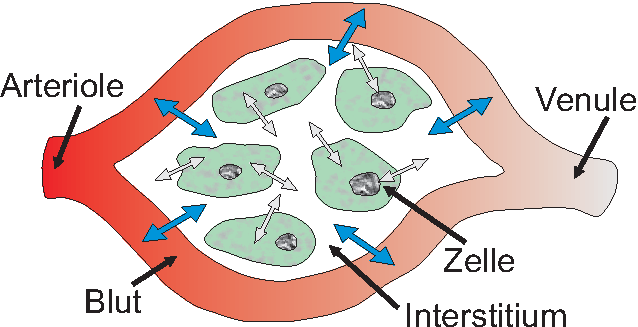
\includegraphics[scale=.75]{images/beispiel1}
   % Die folgende Anweisungen bindet die Grafik nocheinmal zus�tzlich
   % als Dateianhang ein. Das hat den Vorteil, dass sie einfach aus dem pdf zur
   % wieterverwendung extrahierbar ist und der Autor (author) mit angegeben
   % werden kann. Leider ist die Grafik dadurch auch gleich zweimal im pdf
   % enthalten und verbraucht dadurch doppelt Platz.
   % \textattachfile[mimetype=application/pdf,print=false,author=\docauthor,description=\figurename~\ref{fig:beispiel1}]{beispiel1.pdf}{}
  %% Reihenfolge der Befehle wichtig: zuerst die \caption, danach das \label
  \caption{Der Gasaustausch zwischen Blut und Zellen findet auf kapillarer Ebene �ber das Interstitium statt, aus \cite{walter2002}}
  \label{fig:beispiel1}
\end{figure}


Gleichungen werden zentriert und am rechten Rand abschnittsweise nummeriert(z.B. (2.1), (2.2),...; (5.1),
(5.2),...). Ein Beispiel gibt nachfolgende Gl.~\ref{eqn:e_mod_laminar}.
\begin{equation}\label{eqn:e_mod_laminar}
  \dot V = \frac{\pi \, \Delta p \, r^4}{8 \, \eta \, l} =
  G_{Strom} \: \Delta p
\end{equation}

\begin{equation}\label{erster}
    \begin{split}
    a &= b +c \\
      &= e + f
\end{split}
\end{equation}
Man beachte: Bilder haben Bildunterschriften, Tabellen haben Tabellen�berschriften, siehe
\tablename~\ref{tab:beispiel}. Die neuen amtlichen Regeln und Schreibungen der deutschen
Rechtschreibung sind zu beachten.

\begin{table}[!ht]
  \centering
  %% Reihenfolge der Befehle wichtig: zuerst die \caption, danach das \label
  \captionabove{Dies ist eine Tabellen�berschrift}
  \begin{tabular}{l|cr}
                                  Spalte 1 & Spalte 2 & Spalte 3\\
                                  \hhline{|=|==|}
                                  Links & Mitte & Rechts\\
                                  \hhline{---}
                                  eins & zwei & drei
  \end{tabular}
  \label{tab:beispiel}
\end{table}

Auf alle Bilder, Tabellen und Gleichungen ist im Text mindestens einmal zu verweisen (z.B. ... wie
man in \figurename~\ref{fig:beispiel1} erkennt, ....). Die Platzierung der Bilder und Tabellen soll in
unmittelbarer N�he zu diesem (ersten) Textverweis erfolgen.


\subsection{Grundlagen / Stand der Technik}
In einem besonderen Abschnitt sollen die notwendigen theoretischen und praktischen Grundlagen
und Voraussetzungen der Arbeit dargestellt werden. Auf Beweise, ausf�hrliche Ableitungen und
weitergehende Erl�uterungen kann, soweit sie in der Literatur bekannt sind, verzichtet werden.
Umfangreiche Zwischenrechnungen und nebens�chliche Ausarbeitungen sollen im Anhang
untergebracht werden.

\subsection{Durchf�hrung}
In den folgenden Abschnitten sollen die Ergebnisse der Arbeit dargestellt werden. Dabei soll insbesondere
erkennbar sein, was selbst erarbeitet und was evtl. aus welcher anderen Arbeit (Zitat) unmittelbar
entnommen und in die eigene Arbeit integriert wurde. Eine genaue Beschreibung der
erstellten Berechnungen, Programme, Schaltungen oder Konstruktionen und �hnlichem ist
erforderlich. Alle notwendigen Bilder (z.B. in Form von Pl�nen, Diagrammen) und sonstige
Unterlagen sind, soweit sie zur Erl�uterung ben�tigt werden, hier einzuf�gen.

\subsection{Dokumentation von Software}
Die Beschreibung muss so erstellt sein, dass ein sp�terer Benutzer das Programm f�r sein Problem
leicht einsetzen bzw. die f�r ihn notwendigen �nderungen durchf�hren kann. Sie beinhaltet eine
Darstellung der Aufgabe und des Aufbaus des Programmsystems sowie eine Beschreibung der verwendeten
Unterprogramme. Hierbei k�nnen beispielsweise Ablaufdiagramme oder Psudocode f�r die Erkl�rung
sinnvoll verwendet werden. Bei umfangreichen Softwarepaketen mit einem User-Interface kann es
sinnvoll sein, zus�tzlich eine kurze Bedienungsanleitung zu erstellen, die die Verwendung erkl�rt.
Ein Abdruck des gesamten Programmcodes ist nicht notwendig.

Bei der Darstellung des Programmsystems soll ein �berblick �ber die Aufgabe und den Ablauf des
Gesamtsystems gegeben werden. Die Organisation und die Verkn�pfung der Komponenten muss erl�utert
werden. Die notwendigen Ein- und Ausgaben, die Bedeutung der Parameter und evtl. vorhandene
Steuerm�glichkeiten sollen angegeben werden. Oftmals ist es sinnvoll auch die grunds�tzlichen
Ideen, �berlegungen und Randbedingungen, die zu der verwendeten Implementierung gef�hrt haben zu
dokumentieren.

Ein wesentlicher Teil der Softwaredokumentation erfolgt durch Kommentare im Programmtext selbst. So
ist jede Komponente mit einem Header zu versehen, der die verwendeten Ein- und Ausgangsgr��en (in
Format, Wertebereich und Bedeutung), die benutzten und ggf. ver�nderten globalen Variablen, und
eine kurze und pr�gnante Beschreibung der Arbeitsweise enth�lt. Auch im weiteren Verlauf sind
Kommentare m�glichst oft f�r die weitere Erkl�rung der Funktion zu verwenden.


\subsection{Dokumentation von Schaltungen}
Schaltungen von elektrischen Ger�ten werden am g�nstigsten zuerst in einem Blockschaltbild
dargestellt. Die Arbeitsweise von einzelnen, nicht allgemein gebr�uchlichen Schaltungsarten sollte
bei der Beschreibung der Gesamtschaltung besonders hervorgehoben werden. Besonderes Augenmerk ist
auf die Einstell- und Abgleichvorschriften zu legen, um einem sp�teren Benutzer die Verwendung zu
erleichtern. Auch Pr�fvorschriften zur Ermittlung von Fehlern bzw. defekten Bauteilen sind
anzugeben. Im Anhang sind eine vollst�ndige Bauteileliste (inkl. Bezugsquellen), die
Schaltungsauslegungen mit evtl. vorhandenen Layouts f�r gedruckte Platinen, Best�ckungszeichnungen
und Steckerbelegungspl�ne anzugeben. Von wenig gebr�uchlichen Einzelkomponenten (z.B. Spezial-IC's)
sollten relevante Ausz�ge der Datenbl�tter in den Anhang eingef�gt werden.

\subsection{Dokumentation von mechanischen Konstruktionen}
Mechanische Aufbauten sollten in der Arbeit selbst durch Prinzipskizzen nach den Regeln technischer
Zeichnungen (DIN Taschenbuch 2, Normen technisches Zeichnen \cite{DIN_Norm_TZ}) und Fotos
dargestellt werden. Besonderheiten bei der Anfertigung, wie spezielle Fertigungsverfahren,
Zusammenbau und Justiervorschriften, sind gesondert zu erl�utern. Im Anhang sollen ma�stabsgetreue
Einzelteilzeichnungen und Zusammenbauzeichnungen beigef�gt werden. Falls die Durchf�hrung von
Wartungsarbeiten erforderlich ist, muss ein entsprechender Ma�nahmenkatalog enthalten sein.

\subsection{Ergebnisse\label{sec:ergebnisse}}
Im vorletzten Abschnitt sollen die bei der Durchf�hrung der Arbeit gewonnenen Ergebnisse
zusammengefasst dargestellt werden. Besonders wichtig ist eine Wertung und Einordnung der
Ergebnisse. Auch Nicht-Erfolge k�nnen ein Ergebnis sein. Messkurven und Messreihen geh�ren, solange
sie nicht als Beispiel ein spezielles Ergebnis erl�utern, in den Anhang.

\subsection{Zusammenfassung und Ausblick}
Neben einer kurzen Zusammenfassung der wichtigsten Ergebnisse soll in diesem Abschnitt auf
weiterf�hrende Fragestellungen oder noch offene, durch die Arbeit aufgeworfene, Probleme
hingewiesen werden (Umfang maximal 2-3 Seiten).


\section{Umgang mit geistigem Eigentum Dritter}

Nicht zuletzt durch die �ffentliche Diskussion um die Dissertationen einiger Politiker ist das Thema Plagiat und Urheberschaft in der wissenschaftlichen Praxis in den Fokus des Interesses ger�ckt. Hierbei m�ssen zwei Rechtsaspekte voneinander unterschieden werden. Zum einen das Urheberrecht. Hier geht es darum, dass ein Autor bestimmte Rechte an seinem Werk hat und somit bestimmte Bedingungen bei der Publikation eingehalten werden m�ssen, damit die Rechte des Autors nicht verletzt werden, oder er als Ausgleich daf�r kompensiert wird (z.B. durch Lizenzzahlungen).
Der andere Aspekt betrifft die geistige Urheberschaft origin�rer Gedanken. Hier geht es in der wissenschaftlichen Praxis darum kenntlich zu machen, wer der geistige Urheber des geschriebenen Textes ist und welches Ma� an eigener Leistung darin enthalten ist. Nicht zuletzt bei wissenschaftlichen Arbeiten ist dies ja auch ein relevantes Bewertungskriterium. 

Aber nicht nur Doktorarbeiten prominenter Politiker unterliegen diesen Rechtsnormen, auch eine studentische Abschlussarbeit hat die gleichen Anforderungen zu erf�llen. Allerdings findet das Urheberrecht nur beschr�nkt Anwendung, da das Ergebnis der Bachelor- oder Masterarbeit ja nicht �ffentlich publiziert wird und damit die freie Verwendung gestattet ist. Die Frage der geistigen Urheberschaft ist aber in jedem Falle zu beachten.

Zur �berpr�fung der Einhaltung der Rechtsnormen gehen immer mehr Universit�ten dazu �ber, alle Abschlussarbeiten einem automatischen Plagiats-Check durch entsprechende Software zu unterwerfen. An der RWTH Aachen ist dies derzeit nicht verpflichtend, aber erste Pilotprojekte werden hierzu derzeit gestartet. Zudem ist auch zu bedenken, dass selbst wenn ein solcher Check heute noch nicht �berall stattfindet, es nicht auszuschlie�en ist, dass dieser irgendwann in der Zukunft nicht auch retrospektiv durchgef�hrt wird.

Weitere Informationen zum Thema k�nnen beispielsweise in \cite{DFG_richtlinie}, \cite{Uni_Wien} und \cite{Unijournal06_4} gefunden werden. 


\subsection{Literaturzitate}
Bei der Abhandlung einer wissenschaftlichen Arbeit steht man also vor einem Dilemma, dass einerseits gerade das Studium und die Aufarbeitung der Literatur ja ein zentrales Werkzeug der wissenschaftlichen Arbeit ist, andererseits im Text klar kenntlich werden soll, was eine eigene Leistung und was der Anteil Dritter am Ergebnis ist. Hierbei ist es wichtig festzustellen, dass es keineswegs eine Abwertung bedeutet, wenn Quellen Dritter im eigenen Text verwendet werden, vielmehr macht es im Gegenteil deutlich, dass der Autor mit der Materie vertraut ist und den Stand der Technik gut �berblickt. Behauptungen und Fakten, die im Weiteren Verlauf der Arbeit nicht abgeleitet, ermittelt oder bewiesen werden, sollten durch einen Quellenverweis (sog. Belegzitat) ausgestattet werden.

\begin{quote}
... zur Bestimmung der Ordnung eines ARMA Signalfilters kann das sogenannte ''Akaike Information Criterion'' \cite{Akaike1974a} herangezogen werden.
\end{quote}

Davon ausgenommen ist die Beschreibung von Grundlagenwissen, das bei der typischen Leserschaft als bekannt vorausgesetzt werden kann. Daf�r stelle man sich beispielsweise einfach vor, was ein durchschnittlicher Fachstudienkollege wissen w�rde, der keine Abschlussarbeit direkt im gleichen Thema geschrieben hat.

Bei jeder wissenschaftlichen Arbeit wird besonderer Wert auf die vollst�ndige und einheitliche Zitierung fremder Quellen gelegt. Vollst�ndigkeit bedeutet, dass jede Verwendung fremden geistigen Eigentums durch genaue Quellenangabe kenntlich gemacht werden muss. Es ist hierbei zu unterscheiden
zwischen der w�rtlichen, der genauen inhaltlichen und der sinngem��en Wiedergabe. Der w�rtlich �bernommene Text (S�tze, Satzteile, einzelne W�rter) ist durch Anf�hrungszeichen ("`die Axt im \ldots\  erspart den Zimmermann"', aus \cite{Schiller:Tell}) zu kennzeichnen. Dabei darf der Text nicht
ver�ndert werden. Die Auslassung eines oder mehrerer Worte ist durch drei Punkte (\ldots\ ) anzudeuten. Es ist immer der Ursprungstext zu zitieren, nicht etwa das Zitat durch einen anderen (Prim�rzitate statt Sekund�rzitate verwenden). Nur, wenn das Original nicht beschaffbar ist, sollte man hiervon Gebrauch machen. Dann ist aber die Sekund�rliteratur zu referenzieren und auf das Zitat (z.B. zit. nach ...) hinzuweisen.

\begin{quote}\rmfamily\small\itshape
Lange Zitate k�nnen zus�tzlich durch einger�ckten engeren Schriftsatz mit kleinerer, kursiver Schrift (wie mit diesem Satz angedeutet) abgehoben werden.\end{quote}

Werden fremdsprachige Texte in eigener �bersetzung wiedergegeben, so ist dies kenntlich zu machen
("`\ldots\  Text \ldots\ "' �bersetzung aus \cite{Akaike1974a}). Auch die genaue inhaltliche oder die sinngem��e Wiedergabe fremden geistigen Eigentums ist durch unmissverst�ndlichen Quellenverweis kenntlich zu machen.

Die Anwendung der Zitatregeln soll an folgendem Beispiel aus \cite{web_pruschmann} deutlich werden:

\begin{quote}\rmfamily\small\itshape
Mit Hilfe einer Textstelle aus der Publikation ''Geschlecht. Wider die Nat�rlichkeit'' von Heinz-J�rgen Vo� soll verdeutlicht werden, was gemeint ist:

Das Originalzitat: ''Gegen solche ''darwinistischen Schw�rmereien'' der Entwicklung auch von Frauengehirnen auf �hnliche oder gleiche H�he wie die der M�nner, wenn es die gesellschaftlichen Bedingungen endlich zulie�en, regte sich Widerstand, so bei Paul Julius M�bius, der sich energisch gegen die Frauenemanzipation wandte.'' \cite{Voss2011},S. 211

Verwendungsbeispiel 1: Gegen solche ''darwinistischen Schw�rmereien'' der Entwicklung auch von Frauengehirnen auf �hnliche oder gleiche H�he wie die der M�nner, wenn es die gesellschaftlichen Bedingungen endlich zulie�en, regte sich Widerstand, so bei Paul Julius M�bius, der sich energisch gegen die Frauenemanzipation wandte. (Ein klares Plagiat. Es fehlen die Anf�hrungszeichen und die Quellenangabe.)


Verwendungsbeispiel 2: Gegen solche ''darwinistischen Schw�rmereien'' der Entwicklung auch von Frauengehirnen auf �hnliche oder gleiche H�he wie die der M�nner, wenn es die gesellschaftlichen Bedingungen endlich zulie�en, regte sich Widerstand, so bei Paul Julius M�bius, der sich energisch gegen die Frauenemanzipation wandte \cite{Voss2011},S. 211. (Die Quelle wird zwar angegeben, aber die Textpassage wird nicht durch Anf�hrungszeichen als Zitat gekennzeichnet. Es handelt sich ebenso um ein Plagiat.)

Verwendungsbeispiel 3: Gegen solche ''darwinistischen Schw�rmereien'' der Entwicklung von Frauengehirnen auf �hnliche H�he wie bei M�nnern, wenn es die gesellschaftlichen Bedingungen zulie�en, regte sich zum Beispiel bei Paul Julius M�bius Widerstand, der sich entschieden gegen die Frauenemanzipation wandte \cite{Voss2011},S. 211. (Das ist ebenso ein Plagiat. Das Zitat wurde nur geringf�gig abge�ndert, doch es ist noch keine Paraphrase und die �bernommenen Formulierungen m�ssen als Zitat gekennzeichnet werden. Durch das leichte Redigieren der Textstelle entsteht hier sogar der Verdacht einer bewussten T�uschung. Diese Vorgehensweise wird auch Verteidigungsminister zu Guttenberg vorgeworfen.)

Verwendungsbeispiel 4: ''Gegen solche 'darwinistischen Schw�rmereien' der Entwicklung auch von Frauengehirnen auf �hnliche oder gleiche H�he wie die der M�nner, wenn es die gesellschaftlichen Bedingungen endlich zulie�en, regte sich Widerstand, so bei Paul Julius M�bius, der sich energisch gegen die Frauenemanzipation wandte.'' \cite{Voss2011},S. 211. (Hier wird die �bernommene Textstelle korrekt ausgewiesen (Ausf�hrungszeichen) und die entsprechende Quelle gekennzeichnet.)

Verwendungsbeispiel 5: Die Auffassung, dass sich bei entsprechenden gesellschaftlichen Bedingungen Frauengehirne in gleicher Weise entwickeln w�rden, war kein gesellschaftlicher Konsens. Protest kam etwa von Paul Julius M�bius, der ein entschiedener Gegner der Emanzipation der Frauen war \cite{Voss2011},S. 211. (Die Textstelle wurde paraphrasiert und die Quelle des zugrundeliegenden Gedankens korrekt angegeben.)

\end{quote}


Quellenverweise erfolgen durch Kurzinformationen im Text. Diese bestehen aus in den Text
eingef�gten Klammerausdr�cken, in denen z.B. eine zitierte Literaturquelle in Kurzform erw�hnt
wird. Beispiel: (vgl. \cite{Schiller:Tell}, S.6 ff). Anhand des Literaturverzeichnisses muss es
m�glich sein, den Kurztitel wieder zu entschl�sseln.

Soll auf zwei aufeinander folgende Seiten verwiesen werden, ist die erstgenannte Seite mit einem
"`f."' (f�r folgende Seite) zu versehen. Entsprechend steht die Abk�rzung "`ff."' (fort- folgende
Seiten) f�r eine unbestimmte Anzahl von Seiten im Anschluss an die erw�hnte. Statt "`ff."' kann
auch der konkrete Seitenumfang angegeben werden (z.B.: S. 254-286). Bei der Verwendung
englischsprachiger Literatur ist auch die Verwendung der Seitenbezeichnungen "`p."' (f�r page) und
"`pp."' (f�r pages) m�glich. Egal wie zitiert wird, wichtig ist eine gewisse Einheitlichkeit.


Das Literaturverzeichnis darf nur die tats�chlich benutzte Literatur enthalten. Alle aufgef�hrten
Titel m�ssen im Text wenigstens einmal zitiert werden. F�r deutsche Texte gilt sinngem�� der
\LaTeX\ -Zitier-Stil "`alphadin"'. Eine Auswahl der dort definierten Typen ist in
\tablename~\ref{tab:ElementeLiteraturverzeichnis} zu finden. Es sollten nach M�glichkeit nur diese
Dokumenttypen verwendet werden.

Einige Informationen und Referenzen sind mittlerweile nur noch online im Internet erh�ltlich. Da im
allgemeinen nicht sichergestellt werden kann, dass diese Informationen auch Morgen noch in der
verwendeten Art und Weise verf�gbar sind, sollten solche Referenzen nach M�glichkeit vermieden
werden. Dies gilt nicht f�r online-Journals mit eigener ISSN/ISBN Nummer. Diese k�nnen wie eine Zeitschrift referenziert werden.

F�r Verweise auf Webseiten verwendet man am besten den Eintragstyp ''MISC''. Wichtig ist hier neben
dem vollst�ndigem Link auch die Angabe, wann die Seite zuletzt besucht worden ist, siehe
\cite{medit2007}.

\begin{table}%[!ht]
%  \rule[-2mm]{0cm}{2mm} %(wenn der Abstand zu klein wird)
   \centering
   %% Reihenfolge der Befehle wichtig: zuerst die \caption, danach das \label
   \captionabove{Elemente des Literaturverzeichnisses nach \cite{Goossens:LatexBegleiter} }
   \newcolumntype{Y}{>{\footnotesize\RaggedRight\arraybackslash}X}
   \begin{tabularx}{\linewidth}{>{\setlength{\hsize}{.6\hsize}}Y%
   |>{\setlength{\hsize}{1.1333\hsize}}Y%
   >{\setlength{\hsize}{1.1333\hsize}}Y%
   >{\setlength{\hsize}{1.1333\hsize}}Y%
   }
   Typ & Beschreibung & Angaben & optionale Angaben\\
   \hline
   article &  Ein Artikel aus einem wissenschaftlichen Journal oder einer Zeitschrift &
   author, title, journal, year & volume, number, pages, month, note. \\
   book    &  Ein Buch, in dem explizit der Verlag angegeben ist&
   author oder editor, title, publisher, year & volume oder number, series, address, edition, month, note\\
   incol\-lection & Ein Teil eines Buches mit eigenem Titel &
   author, title, booktitle, publisher, year & editor, volume oder number, series, type, chapter, pages, address, edition, month, note.\\
   inprocee\-dings & Ein Artikel in einem Konferenzband &
   author, title, booktitle, year& editor, volume oder number, series, pages, address, month, organization, publisher, note.\\
   manual & Technische Dokumentation &
   title&author, organization, address, edition, month, year, note\\
   tech\-re\-port & Ein Bericht, ver�ffentlicht von einer Hochschule oder einer anderen Institution; normalerweise eine nummerierte Ausgabe in einer Reihe.&
   author, title, institution, year&type, number, address, month, note\\
   unpub\-lish\-ed & Ein Dokument, das Autor und Titel hat, aber nicht ver�ffentlicht wurde.& author, title, note& month, year\\
   masters\-the\-sis & Eine Diplomarbeit & author, title, school, year & type, address, month, note\\
   phd\-the\-sis & Eine Doktorarbeit &author, title, school, year & type, address, month, note\\
   misc & alles sonst & author, title, year & howpublished\\
   \end{tabularx}
   \label{tab:ElementeLiteraturverzeichnis}
\end{table}

\clearpage

Die verwendeten Quellen sind in alphabetischer Reihenfolge nach Verfassern bzw. Herausgebern bzw.
bei fehlender Verfasserangabe nach Sachtiteln sortiert aufzuf�hren. Das Literaturverzeichnis muss
komplette, ungek�rzte Quellenangaben enthalten. Die genaue Schreibweise entnimmt man am besten der
Beispielbibliografie am Ende dieses Dokumentes.

Folgenden Textverweise werden beispielsweise im \LaTeX\ -Zitier-Stil "`alphadin"' verwendet:
\begin{quotation}
Artikel in Zeitschriften mit einem Autor \cite{Akaike1974a}, mit mehreren Autoren
\cite{Aschoff1999a}, Artikel in Konferenzb�nden mit mehreren Autoren \cite{Walter12.-16.6.1998a},
B�cher mit einem Autor \cite{Schiller:Tell}, mit mehreren Autoren \cite{Goossens:LatexBegleiter},
Dissertationen mit einem Autor (deutsch) \cite{walter2002}
\end{quotation}

%\clearpage

\subsection{Bildzitate}
Auch Bilder unterliegen dem Urheberrecht und sind bei ihrer Verwendung eindeutig zu kennzeichnen. So lange die Abschlussarbeit nicht ver�ffentlicht wird, ist die Verwendung Bilder Dritter erlaubt und lizenzfrei. Die Kenntlichmachung der Urheberschaft ist aber zwingend notwendig.

\begin{itemize}
\item Wird ein Bild ohne oder nur mit geringen Ver�nderungen verwendet, so ist die Quelle entweder im Bild oder durch Quellenverweis in der Bildunterschrift kenntlich zu machen.
\item Wird das Bild in Teilen ver�ndert, so ist die Beziehung zum urspr�nglichen Bild entweder im Bild oder durch Quellenverweis in der Bildunterschrift kenntlich zu machen. z.B. durch: ... Nachgezeichnet nach \cite{walter2002}, ... Ver�ndert nach \cite{Aschoff1999a}, ... Modifiziert nach \cite{walter2002}
\item Wird das Bild aus Daten einer Ver�ffentlichung Dritter erzeugt, so liegt gem�� Urheberrecht sicher ein eigenes Werk vor. Trotzdem sollte die Quelle benannt werden, damit deutlich wird, woher die originalen Daten stammen (sog. Belegzitat). z.B. durch: ... nach Daten aus \cite{Akaike1974a}
\end{itemize}




\section{Anhang}

Die mathematischen Berechnungen und Beweise auf die in dem Abschnitt Grundlagen verzichtet wurde,
sind im Anhang ausf�hrlich darzustellen. In einem Abschnitt f�r Pl�ne sind vollst�ndige
Konstruktionszeichnungen, Montage- und Demontagepl�ne, Wartungspl�ne, Schaltpl�ne,
Best�ckungslisten usw. f�r die erstellten Ger�te und Schaltungen anzuf�gen. Im Anhang sind, soweit
nicht im Text bereits erfolgt, s�mtliche Messkurven und Messreihen, auf die sich die Ergebnisse
st�tzen, vollst�ndig anzugeben. Sollte dies auf Grund gro�er Komplexit�t nicht m�glich sein, so ist
zumindest eine relevante Auswahl zu treffen. Hilfreich ist auch eine Dokumentation des
Ablagesystems der Messdaten (z.B. geordnet nach Versuchstagen, Testobjekt, o.�.). Auch geforderte
Bedienungsanleitungen, Praktikumsbeschreibungen u.�. sollen im Anhang untergebracht werden.



\section{schriftliche Erkl�rung}
Bei jeder wissenschaftlichen Arbeit zum Zwecke der Erlangung einer formalen Qualifikation ist eine eidesstattliche Versicherung
abzugeben.

Der Vordruck f�r diese Erkl�rung ist bereits in der \LaTeX\ Vorlage f�r dieses Dokument enthalten.

\section{Erstellung / Speicherung von Grafiken\label{sec:grafik}}

Grafiken k�nnen im Prinzip mit jedem daf�r geeigneten Programm erstellt werden. F�r Vektorgrafiken
bevorzugt werden sollten aber XFig und CorelDraw, f�r Pixelgrafiken Gimp, Corel Photo Paint oder
Paintshop Pro. Die Grafiken sollten f�r Text in der Grafik ausschlie�lich Standardschriftarten in
der Gr��e 12pt verwenden.

Das Originalformat sollte erhalten bleiben und bei vom Standard abweichender Software dokumentiert
werden. Alle Grafiken sollten auch im Original auf dem Archiv-Datentr�ger enthalten sein. Da die
Originalformate selten f�r die direkte Verwendung in einer Textverarbeitung / Pr�sentationsprogramm
(OpenOffice Writer, Wordperfect, Word / Powerpoint) oder einem Satzsystem (pdf\LaTeX\ )
geeignet sind, m�ssen von jeder Grafik zus�tzliche Importversionen erstellt werden.

F�r Vektorgrafiken sind dies pdf (pdf\LaTeX\ ) und wmf (der Rest). Pixelgrafiken (Scans,
Fotos) sollten bevorzugt im verlustlos komprimierenden png-Format abgelegt werden, um
Kompressionsartefakte zu vermeiden. Dies gilt speziell f�r Grafiken mit "`scharfen"' Kanten wie
z.B. Screenshots. jpeg sollte nur in Ausnahmef�llen f�r Fotografien verwendet werden. Ein
verlustlos (FlateEncode) komprimiertes pdf der Pixelgrafik w�re von Vorteil, da png Bilder
pdf\LaTeX\  Durchl�ufe stark verlangsamen k�nnen.

Diese Importversionen sollten nach M�glichkeit direkt nach der Fertigstellung einer Grafik erzeugt
werden, sp�testens aber nach Fertigstellung eines Artikels / Dokuments. Da die Konvertierung
oftmals mit einigen Problemen verbunden ist, sollten s�mtliche Importversionen einer Grafik
�berpr�ft werden. Vektorformate wie pdf und wmf definieren neben den r�umlichen Abmessungen der
eigentlichen Grafikobjekte (Buchstaben, Linien, ...) auch eine Seitengr��e, auf der diese
dargestellt werden. Deshalb ist darauf zu achten, dass die Seitengr��e exakt mit der maximalen
Objektausdehnung �bereinstimmt und nicht eine wenige cm gro�e Grafik auf einem sonst fast leeren A4
Blatt entsteht. Eventuell notwendige Abstandshalter zwischen Grafiken und Text sind mit den Mitteln
der Textverarbeitung / des Satzsystems zu realisieren und nicht durch einen wei�en Rand o. �. in
der Grafik.

Die notwendige "`toolchain"' f�r die Konvertierungen befindet sich im "`fliegenden"' Aufbau, bzw.
ist st�ndigen Ver�nderungen unterworfen. Hilfestellung bei der Erzeugung der Grafikformate bietet
unter anderem das instituseigene Wiki Informationssystem.

\chapter{PDF und Postscript}\label{sec:pdfundps}

Das korrekte Erzeugen von Dateien, die internationalen Standards der Druckindustrie gen�gen, ist
eine nicht unbedingt triviale Aufgabe. Um eine m�glichst lange Verwendbarkeit der Dateien zu
gew�hrleisten, soll im folgenden eine Hilfestellung gegeben werden.

\section{Dateiformat}
Postscript ist eigentlich eine vollwertige Programmiersprache, die urspr�nglich (von der Firma Adobe) f�r die Programmierung von Druckern entwickelt wurde.
Eine Postscript Datei ist nichts anderes als ein Programm f�r einen Postscript f�higen Drucker, das normalerweise zur Ausgabe einer bedruckten Seite f�hrt. Fr�her verf�gten Postscript Drucker �ber vergleichsweise schnelle Prozessoren und wurden daher auch zur L�sung von Rechenaufgaben (mit einem Postscript Programm) zweckentfremdet.

Mit Ghostscript gibt es seit l�ngerem einen frei verf�gbaren Postscript Interpreter, der es m�glich macht Postscript Dateien auf einem normalen Rechner auszuf�hren und das Ergebnis auf dem Bildschirm, anstelle von Papier, darzustellen. Alternativ kann die Ausgabe auch in einem anderen Dateiformat (z.B. pdf oder png) erfolgen, was zur Konvertierung genutzt werden kann.

PDF (ebenfalls von der Firma Adobe) erm�glicht die layoutgetreue Abspeicherung von Seiten, z.B. f�r die sp�tere Ausgabe auf einem (beliebigen) Drucker. Das Konzept von PDF orientiert sich stark an Postscript, stellt aber keine vollwertige Programmiersprache dar, sondern beschr�nkt sich auf die Funktionen, die zur Ausgabe von Grafiken, Texten, Zeichnungen und �hnlichem auf einer Seite notwendig sind. Der bei neueren Versionen hinzugekommene JavaScript Dialekt relativiert diese Einschr�nkung allerdings wieder.

Die Weiterentwicklung von Postscript und PDF verl�uft parallel. Neuerungen flie�en sowohl von Postscript nach PDF als auch umgekehrt.

F�r den Anwender ist es am einfachsten sich sowohl Postscript als auch PDF als eine Sammlung von Objekten vorzustellen.
Objekte k�nnen z.B. Zeichenobjekte (Grafiken, Textzeichen, Linien usw.) sein, die auf einer Seite (bzw. einem Seitenobjekt) positioniert sind.
Ein Objekt kann aber genausogut ein Dateianhang �hnlich einem Mailanhang sein, der sich auf einem Datentr�ger speichern l�sst oder eine spezielle Schriftart (z.B. eine mathematische Symbolschrift).

\subsection{PDF Versionen\label{sec:pdfversionen}}
F�r PDF Dateien existieren verschiedene Standards und Versionen. Die Versionen werden von der Fa.
Adobe vergeben. Bisher sind u.a. die Versionen 1.3 (f�r Acrobat~4), 1.4 (f�r Acrobat~5), 1.5 (f�r Acrobat~6) und 1.6 (f�r Acrobat~7) bekannt. F�r den Zweck der Archivierung und Reproduktion reicht bereits Version 1.3 aus.

Die gro�e Flexibilit�t von Postscript bzw. PDF hat leider nicht nur Vorteile.
Ein Problem ist z.B. die Einbettung bzw. das unterlassen der Einbettung der verwendeten Schriften. Der Ersteller eines Dokuments kann seine PDF Datei ohne Probleme lesen, da alle verwendeten Schriftarten auf seinem Rechner vorhanden sind. Sein Betreuer oder auch der Copyshop, der die fertige Arbeit drucken soll hat aber nicht zwangsl�ufig dieselben Schriftarten installiert. Der PDF Betrachter bzw. der Drucker ersetzt dann die Schrift durch eine m�glichst �hnliche Schrift. Das reicht aus, um den Text lesen zu k�nnen, sieht aber meistens sehr schlecht aus.

In der Drucktechnik wird daher der PDF/X-3 Standard verwendet und ist sogar in einer ISO Richtlinie (ISO 15930-3) definiert. Das eigentliche Dateiformat entspricht PDF Version 1.3, schreibt aber u.a. vor, dass alle verwendeten Schriftarten eingebettet sein m�ssen. Das oben dargestellte Problem kann damit nicht mehr auftreten.

\section{Grafiken in PDF Dateien\label{sec:grafikenimpdf}}
In einem Dokument enthaltene Grafiken (s. Abschnitt~\ref{sec:grafik}) werden als Grafikobjekte in ein PDF integriert. Vektorgrafiken setzen sich normalerweise aus vielen kleinen Zeichenelementen (Linien, Kurven, Kreise, Buchstaben usw.) zusammen.
Pixelgrafiken k�nnten theoretisch aus vielen kleinen gef�llten Quadraten zusammengesetzt werden. Das w�re allerdings eine enorme Platzverschwendung. Daher gibt es in PDF spezielle Objekttypen f�r komprimierte Pixelgrafiken.
Die Kompression kann entweder verlustbehaftet (jpeg-Verfahren, im PDF als DCTEncode bezeichnet) oder verlustfrei (zip-Verfahren, im PDF als FlateEncode bezeichnet und noch einige weitere, seltener verwendete Verfahren) erfolgen. Die jpeg-Kompression ist gut f�r Fotos, da diese auf eine ertr�gliche Gr��e komprimiert werden und die Kompressionsartefakte kaum auffallen. Die zip-Kompression bietet sich f�r Bilder mit scharfen Kanten (z.B. Bilder mit viel Text und Screenshots) an. Derartiges Bildmaterial w�rde von jpeg zum Einen nicht so effizient komprimiert, zum Anderen sehen die entstehenden Artefakte nicht sch�n aus und k�nnen kleine Beschriftungen sogar komplett unlesbar machen. Bilder aus Matlab k�nnen mit dem Tool "`ConvertPlot4Publication"' erzeugt werden. Dieses Tool ist im Internet zu finden.

\section{Postscript und PDF erzeugen}
\subsection{Anforderungen}
Es existieren eine Vielzahl von Softwarel�sungen, um eine PDF
Datei zu erzeugen. Unabh�ngig davon ist folgendes zu beachten:
\begin{quote}
  PDF Dateien der Arbeiten sollten dem PDF/X-3 Standard (s. Abschnitt~\ref{sec:pdfversionen}) entsprechen
\end{quote}
Zur �berpr�fung, ob ein PDF Dokument dem PDF/X-3 Standard entspricht, kann das freeware Tool
PDF/X-3 Inspector (\url{www.pdfx3.org}) verwendet werden. Einige Probleme, wie nicht eingebettete
Schriftarten k�nnen damit auch noch nachtr�glich korrigiert werden. Leider funktioniert es nur in
Zusammenhang mit dem kommerziellen Adobe Acrobat (Version~5 oder h�her) und nicht mit dem Acrobat
Reader.

pdf\LaTeX\  (s. Abschnitt~\ref{sec:pdfmitlatex}) ist eine gute M�glichkeit PDF Dateien zu
erzeugen. Leider entsprechen diese nicht zwangsl�ufig dem PDF/X-3 Standard. Wird die von Medit zur
Verf�gung gestellte Vorlage ohne gr��ere Ver�nderungen verwendet, und beschr�nkt sich die
Inkompatibilit�t auf die gleichen Elemente, wie in diesem Dokument, so ist eine Abweichung vom
PDF/X-3 Standard m�glich. Auf keinen Fall darf aber eine in der Arbeit verwendete Schriftart
fehlen. Ebenso muss darauf geachtet werden, dass alle in PDF Bildern verwendete Schriften korrekt eingebettet sind.

\subsection{\LaTeX\label{sec:pdfmitlatex}}
\TeX\  bzw. das auf \TeX\  aufsetzende \LaTeX\  ist deutlich �lter als Postscript
und PDF, war aber lange Zeit ausserhalb der "`Universit�ren Welt"' unbekannt. Die von \LaTeX\ 
erzeugten DVI Dateien beschreiben ebenfalls die layoutgetreue Positionierung von Zeichenobjekten
auf einer Seite (allerdings ohne deren Inhalt). Daher ist es technisch relativ einfach aus einer
DVI Datei eine Postscript oder PDF Datei zu erzeugen. Mit pdf\LaTeX\  gibt es inzwischen auch
eine M�glichkeit direkt PDF Dateien zu erzeugen.

\subsection{Windows Programme}
Im Gegensatz zu pdf\LaTeX\  ist die PDF Erstellung bei anderen Textverarbeitungsprogrammen im
allgemeinen nicht so direkt m�glich. Dort muss der Umweg �ber den Ausdruck des Dokuments in eine
Datei beschritten werden.

In Windows basierenden Systemen kann dazu ein Postscript Druckertreiber (z.B. f�r einen HP C
LaserJet 4500-PS an FILE:) installiert werden. Zus�tzlich m�ssen folgende Einstellungen nach der
Installation vorgenommen werden:
\begin{itemize}
                \item Papier/Ausgabe: "`Papiergr��e"' $=$ "`A4"'
                \item Grafik: "`TrueType-Schriftarten"' $=$ "`Als Softfont in den Drucker laden"'
                \item Optionen f�r Dokument, PostScript-Optionen:
                      \begin{itemize}
                        \item "`PostScript-Ausgabeoption"' $=$ "`Portabilit�t optimieren"'
                        \item "`PostScript-Sprachebene"' $=$ "`2"'
                        \item "`TrueType-Downloadoption"' $=$ "`Umriss"' (bewirkt Einbettung als Type~1 Font)
                      \end{itemize}
\end{itemize}

Dann kann dieser Drucker wie jeder andere Drucker verwendet werden. Anstelle eines Ausdrucks wird
eine Postscript Datei erzeugt. Im Dateinamensdialog sollte die Datei-Endung .ps (f�r PostScript)
verwendet werden.

F�r die automatisierte Erstellung einer PDF Datei eignet sich z.B. FreepdfXP
({\url{http://freepdfxp.de}}). Dieses installiert auf Microsoft Betriebssystemen (Windows 2000 /
XP) einen Drucker, der dann anstelle von Postscript Dateien PDF Dateien erstellt. Die Installation
und Konfiguration des o.g. Druckertreibers ist aber nach wie vor notwendig, weil FreepdfXP intern
eigentlich nichts anderes macht, als die vom Druckertreiber erstellte Postscript Datei in ein PDF
zu konvertieren und erst dieses abzuspeichern.

Ein Problem vieler Textverarbeitungsprogrammen (z.B. Winword) ist die Abh�ngigkeit des
Seitenlayouts vom ausgew�hlten Drucker. Deshalb wird \emph{dringend} empfohlen zu Anfang den o.g.
Drucker auszuw�hlen und nicht mehr zu �ndern. Ansonsten muss das gesamte Layout nochmals auf
korrekten Seitenumbruch und verschobene Objekte kontrolliert werden. F�r den Ausdruck einer
Postscript Datei auf einem nicht Postscript Drucker, kann unter Windows die Kombination aus
Ghostscript und Ghostview (\url{http://www.cs.wisc.edu/\%7Eghost/}) verwendet werden.

\subsection{Adobe Acrobat}
Das kommerzielle Programm Adobe Acrobat stellt sicherlich den Standard f�r die Erzeugung von PDF Dateien dar. Auch hier wird ein Druckertreiber installiert, den jedes Windows-Programm verwenden kann. Zus�tzlich besteht mit dem Acrobat Distiller die M�glichkeit Postscript Dateien in PDF umzuwandeln.
Bei Auswahl der entsprechenden Optionen ist die Erstellung eines PDF/X-3 konformen PDF Dokuments m�glich. Am Lehrstuhl sind einige Lizenzen des Programms verf�gbar, so dass zur Abgabe am besten eine Postscript Datei erzeugt wird, die dann in Zusammenarbeit mit dem Betreuer in ein PDF/X-3 konformes Dokument umgewandelt wird.
Leider behandelt Acrobat die Kompression von in das Dokument eingebetteten Pixelbildern (s. Abschnitt~\ref{sec:grafikenimpdf}) in der Standardeinstellung global. Das heisst s�mtliche Pixelgrafiken werden mit demselben Verfahren komprimiert. Befinden sich sowohl Fotos als auch Scrennshots o.�. im Dokument, wird entweder das Dokument sehr gross (verlustlose Kompression aller Bilder) oder die Screenshots werden sehr unansehlich (verlustbehaftete Kompression).
Vermutlich kann dieses Verhalten auch lokal beeinflusst werden, zur Zeit ist daf�r aber kein konkreter L�sungsweg bekannt.


\chapter{Seminarvortrag}

�ber die angefertigte Arbeit ist ein Vortrag von typischerweise 15 Minuten in m�glichst freier Rede
zu halten. Der Vortrag soll sich an ein sachkundiges Publikum ohne Spezialkenntnisse wenden. Er
muss daher vor allem die Problemstellung, den L�sungsansatz und die Ergebnisse klar darlegen,
braucht aber nur wenige Detailinformationen zu enthalten. Es soll hier eine Darstellung der Aufgabe
oder auch nur eines Teilbereichs der Aufgabe, aber kein T�tigkeitsbericht geboten werden. Ein
einziges gut ausgearbeitetes Beispiel kann oft mehr zeigen als eine gro�e Anzahl von Fakten, die
wegen der gedr�ngten Information vom Zuh�rerkreis in der kurzen Zeit nicht verstanden werden
k�nnen.

Im Anschluss an den Vortrag k�nnen Ger�te und Versuche dem Zuh�rerkreis vorgef�hrt werden.

\section{Gliederung}
Die Gliederung ist zu Beginn des Vortrags anzugeben und in kurzer Form zu erl�utern. W�hrend des
Ablaufs soll zur Orientierungshilfe immer auf den behandelten Gliederungspunkt hingewiesen werden.

\section{Anzahl der Folien}
Wie erw�hnt soll der Vortrag insgesamt 15 Minuten dauern. Zur Absch�tzung der Vortragsdauer kann
man ungef�hr 1 - 2 Minuten zur Erl�uterung einer beschriebenen Folie ansetzen. Der gesamte Vortrag
sollte somit nicht mehr als 12 Folien umfassen (inklusive Titel und Gliederung).

\section{Folien}
Im allgemeinen erfolgt die Darstellung als elektronische Pr�sentation auf den Computer. Zur
Erstellung von Vortragsfolien existieren eine Reihe verschiedener Programme, wie z.B. Microsoft
Powerpoint, CorelDraw, aber auch mit \LaTeX\  erzeugte Postscript und PDF Dokumente k�nnen f�r
einen Vortrag genutzt werden. Im Rahmen der M�glichkeiten werden vom Fachgebiet die notwendigen
Ger�te f�r die Pr�sentation (z.B. Beamer, Computer) zur Verf�gung gestellt. Eine Designvorlage f�r
Powerpoint und \LaTeX\  wird vom Institut zur Verf�gung gestellt.

Bei der Darstellung ist darauf zu achten, dass die verwendeten Schriften 16pt nicht unterschreiten.
An s�mtlichen Diagrammen sind die dargestellten Gr��en mit Wort, Zeichen und Dimension anzugeben.
Multimedia Effekte (wie z.B. Ton oder Videos) k�nnen richtig angewendet gro�e Wirkung erzielen,
allerdings nur, wenn sie der Darstellung von Information dienen. Auch die Animation von Grafiken
und Schrift sollte so sparsam wie m�glich eingesetzt werden. Bei der Auswahl von Farben (z.B. f�r
Schriften, Hintergrund und Hervorhebung) sollte darauf geachtet werden, nicht zu viele verschiedene
Typen zu verwenden. Hilfe gibt auch hier die Folienvorlage des Instituts.

Bei der Gestaltung der Folien empfiehlt sich die Verwendung von Bildern anstelle langer
zusammenh�ngender Textpassagen:
\begin{quote}\rmfamily\small\itshape
"`Ein Bild sagt mehr als 1000 Worte"'
\end{quote}

\section{Probevortrag}
Es empfiehlt sich, den Vortrag mehrfach probeweise zu Hause (und evtl. vor dem Betreuer) zu halten
und dabei laut zu sprechen. Anfangs wird die Dauer noch mehr als doppelt so lange sein, mit
fl�ssigerem Vortrag soll dann aber die angestrebte Vortragsdauer erreicht werden. Anfangs empfiehlt
es sich auch zu jeder Folie einige Stichpunkte auf einen Handzettel zu notieren, an denen man sich
w�hrend des Vortrags orientieren kann.

\chapter{Unfallversicherungsschutz f�r Studenten}
Die Anfertigung von Studien- und Diplomarbeiten bzw. Bachelor- und Masterarbeiten innerhalb der Hochschule f�llt unter den Schutz der
gesetzlichen Unfallversicherung. Arbeiten au�erhalb des organisatorischen Verantwortungsbereiches
der Universit�t gelten als privat, auch wenn sie studien- und lehrstoffbezogen sind. Dies gilt f�r
Arbeiten im h�uslichen Bereich und f�r externe Arbeiten. Bei externen Arbeiten
ist darauf zu achten, dass die betreffende Firma die gesetzliche Unfallversicherung gew�hrt.


%**********
%* Anhang *
%**********

\cleardoublepage
\appendix
\chapter{Latex Nutzung}
\section{Latex DO's \& DON'Ts}
						
Zum richtigen Umgang mit \LaTeX wird die PDF-Datei "`l2tabu"' empfohlen. In ihr sind die wichtigsten Regeln im Umgang mit \LaTeX und dem Koma-Script zusammengefasst (\url{www.mast.queensu.ca/~andrew/LaTeX/latex-dos-and-donts.pdf}).




%********************************************************************************
% Da nicht bei allen Installationen das package pgfplots dabei ist, ist das Matlab Beispiel auskommentiert.
% F�r eine Benutzung muss der folgende Blockkommentar und im Header 
% der Kommentar bei dem package{tikz,pgfplots} entfernt werden.  
%********************************************************************************

\section{Matlab-Einbindung}

Zur Einbindung von Matlab-Plots in \LaTeX\  sollte "`ConvertPlot4Publication"' verwendet werden. Dieses Tool kann im Internet runter geladen werden. Google hilft weiter.


%**********************************************************
% Literaturverzeichnis (hier muss nichts ge�ndert werden) *
%**********************************************************

\bibliographystyle{alphadin}    %\bibliographystyle{} plain dinat
\bibliography{literatur}%


\end{sloppypar}
\end{document}
